% End-of-outbreak decision-making under superspreading and onset-date delays.
%
% Methods and results. Build with the Snakemake `report` rule, or by hand:
%
%     latexmk -pdf -cd report/report.tex
%
% EVERY NUMBER IN THIS DOCUMENT IS \resultnum{...}, and nothing else. The values come from
% ../results/report_numbers.tex, which scripts/run_report_numbers.py generates from the files
% the tier-2 pipeline rules wrote. Do not type a result into the prose: an unknown key is a
% compile error, but a stale literal is invisible. The only numbers written out by hand are
% the ones that are *inputs* rather than results -- and those are macros too, so that changing
% config/config.yaml changes the methods section.
%
% Appendix B is where the repository lives. Keep implementation detail there and out of the
% methods: the body should read as a paper, not as a description of this codebase.

\documentclass[11pt,a4paper]{article}

\usepackage[T1]{fontenc}
\usepackage{lmodern}
\usepackage[margin=2.4cm]{geometry}
\usepackage{amsmath}
\usepackage{amssymb}
\usepackage{amsthm}
\usepackage{graphicx}
\usepackage{booktabs}
\usepackage[font=small,labelfont=bf]{caption}
\usepackage{enumitem}
\usepackage{microtype}
\usepackage{xcolor}
\definecolor{linkcolour}{rgb}{0.10,0.25,0.55}
\usepackage[colorlinks=true,allcolors=linkcolour]{hyperref}
% The prose carries long unbreakable tokens -- repository paths and \resultnum expansions such
% as "0.38 (0.23--0.63)" -- so give the line breaker a little room rather than leaving overfull
% boxes in the margin.
\emergencystretch=1.5em

\setlist[itemize]{itemsep=2pt,topsep=4pt,parsep=0pt}

\theoremstyle{plain}
\newtheorem{proposition}{Proposition}
\theoremstyle{definition}
\newtheorem*{remark}{Remark}

% Repository paths, which are long and would otherwise overflow the measure. \nolinkurl breaks
% them at the slashes and takes underscores verbatim, so a path is written exactly as it is.
\newcommand{\file}[1]{\texttt{\nolinkurl{#1}}}

% --- the results macros --------------------------------------------------------------------
%
% \resultnum{key} expands to a number computed by the pipeline. An unknown key raises a LaTeX
% error rather than printing nothing, so a renamed model or a deleted analysis stops the build.
\makeatletter
\newcommand{\defresultnum}[2]{\expandafter\gdef\csname resultnum@#1\endcsname{#2}}
\newcommand{\resultnum}[1]{%
  \ifcsname resultnum@#1\endcsname
    \csname resultnum@#1\endcsname
  \else
    \GenericError{}{Unknown result key: #1}{}%
      {No such key in results/report_numbers.tex. Re-run the report_numbers rule, or fix the
       key. Numbers are never written into the prose by hand.}%
  \fi
}
\makeatother
% Generated by scripts/run_report_numbers.py -- do not edit.
%
% Every number report/report.tex quotes, keyed for \resultnum. Read from:
%   data/equateur_2018_onsets.csv
%   results/naive_models_fixed_k/dlo_posterior.nc
%   results/naive_models_fixed_k/dlo_rac.csv
%   results/naive_models_fixed_k/model_evidence.json
%   results/naive_models_fixed_k/sse_posterior.nc
%   results/naive_models_fixed_k/sse_rac.csv
%   results/naive_models_fixed_k/ssi_posterior.nc
%   results/naive_models_fixed_k/ssi_rac.csv
%   results/naive_models_estimated_k/dispersion_posteriors.json
%   results/naive_models_estimated_k/dlo_posterior.nc
%   results/naive_models_estimated_k/dlo_rac.csv
%   results/naive_models_estimated_k/model_evidence.json
%   results/naive_models_estimated_k/sse_posterior.nc
%   results/naive_models_estimated_k/sse_rac.csv
%   results/naive_models_estimated_k/ssi_posterior.nc
%   results/naive_models_estimated_k/ssi_rac.csv
%   results/onset_models_fixed_k/model_evidence.json
%   results/onset_models_fixed_k/sse_posterior.nc
%   results/onset_models_fixed_k/sse_rac.csv
%   results/onset_models_fixed_k/sse_so_posterior.nc
%   results/onset_models_fixed_k/sse_so_rac.csv
%   results/onset_models_fixed_k/ssi_posterior.nc
%   results/onset_models_fixed_k/ssi_rac.csv
%   results/onset_models_fixed_k/ssi_so_posterior.nc
%   results/onset_models_fixed_k/ssi_so_rac.csv
%   results/onset_models_estimated_k/dispersion_posteriors.json
%   results/onset_models_estimated_k/model_evidence.json
%   results/onset_models_estimated_k/sse_posterior.nc
%   results/onset_models_estimated_k/sse_rac.csv
%   results/onset_models_estimated_k/sse_so_posterior.nc
%   results/onset_models_estimated_k/sse_so_rac.csv
%   results/onset_models_estimated_k/ssi_posterior.nc
%   results/onset_models_estimated_k/ssi_rac.csv
%   results/onset_models_estimated_k/ssi_so_posterior.nc
%   results/onset_models_estimated_k/ssi_so_rac.csv
%
% 488 entries.
\defresultnum{data.days}{111}
\defresultnum{data.ertarrivaldate}{8 May 2018}
\defresultnum{data.ertarrivalday}{33}
\defresultnum{data.firstdate}{5 April 2018}
\defresultnum{data.firstday}{0}
\defresultnum{data.lastonsetdate}{2 June 2018}
\defresultnum{data.lastonsetday}{58}
\defresultnum{data.maxdailyonsets}{6}
\defresultnum{data.onsetdays}{31}
\defresultnum{data.postertcases}{26}
\defresultnum{data.preertcases}{28}
\defresultnum{data.referencedate}{4 July 2018}
\defresultnum{data.referenceday}{90}
\defresultnum{data.totalcases}{54}
\defresultnum{data.withdrawaldate}{24 July 2018}
\defresultnum{data.withdrawalday}{110}
\defresultnum{delays.alternativeserialinterval.mean}{19.46}
\defresultnum{delays.alternativeserialinterval.sd}{6.08}
\defresultnum{delays.alternativeserialinterval.variance}{36.97}
\defresultnum{delays.discrepancy}{0.00070}
\defresultnum{delays.incubation.mean}{11.40}
\defresultnum{delays.incubation.sd}{8.10}
\defresultnum{delays.incubation.variance}{65.61}
\defresultnum{delays.maxlag}{110}
\defresultnum{delays.serialinterval.mean}{15.30}
\defresultnum{delays.serialinterval.sd}{9.30}
\defresultnum{delays.serialinterval.variance}{86.49}
\defresultnum{delays.tolerance}{0.02}
\defresultnum{delays.tost.mean}{3.90}
\defresultnum{delays.tost.sd}{4.57}
\defresultnum{delays.tost.variance}{20.88}
\defresultnum{naivemodelsestimatedk.chains}{4}
\defresultnum{naivemodelsestimatedk.diagnostics.divergences}{0}
\defresultnum{naivemodelsestimatedk.diagnostics.maxrhat}{1.00}
\defresultnum{naivemodelsestimatedk.diagnostics.minbulkess}{4074}
\defresultnum{naivemodelsestimatedk.dlo-vs-sse.medianratio}{0.75}
\defresultnum{naivemodelsestimatedk.dlo-vs-sse.overlap}{0.589}
\defresultnum{naivemodelsestimatedk.dlo-vs-sse.probabilitygreater}{0.219}
\defresultnum{naivemodelsestimatedk.dlo-vs-ssi.medianratio}{2.69}
\defresultnum{naivemodelsestimatedk.dlo-vs-ssi.overlap}{0.094}
\defresultnum{naivemodelsestimatedk.dlo-vs-ssi.probabilitygreater}{0.990}
\defresultnum{naivemodelsestimatedk.dlo.evidencegain}{\ensuremath{+3.90}}
\defresultnum{naivemodelsestimatedk.dlo.k.interval}{0.378 (0.230--0.629)}
\defresultnum{naivemodelsestimatedk.dlo.k.lower}{0.230}
\defresultnum{naivemodelsestimatedk.dlo.k.median}{0.378}
\defresultnum{naivemodelsestimatedk.dlo.k.upper}{0.629}
\defresultnum{naivemodelsestimatedk.dlo.logevidence}{\ensuremath{-93.2}}
\defresultnum{naivemodelsestimatedk.dlo.logevidencese}{0.002}
\defresultnum{naivemodelsestimatedk.dlo.probability}{\ensuremath{2\times 10^{-4}}}
\defresultnum{naivemodelsestimatedk.dlo.rac.final}{0.032}
\defresultnum{naivemodelsestimatedk.dlo.rac.mcse}{0.0012}
\defresultnum{naivemodelsestimatedk.dlo.rac.mcselate}{0.0012}
\defresultnum{naivemodelsestimatedk.dlo.rac.reference}{0.429}
\defresultnum{naivemodelsestimatedk.dlo.rac01.date}{never}
\defresultnum{naivemodelsestimatedk.dlo.rac01.day}{never}
\defresultnum{naivemodelsestimatedk.dlo.rac05.date}{21 July 2018}
\defresultnum{naivemodelsestimatedk.dlo.rac05.day}{107}
\defresultnum{naivemodelsestimatedk.dlo.rpost.interval}{0.59 (0.33--1.05)}
\defresultnum{naivemodelsestimatedk.dlo.rpost.lower}{0.33}
\defresultnum{naivemodelsestimatedk.dlo.rpost.median}{0.59}
\defresultnum{naivemodelsestimatedk.dlo.rpost.upper}{1.05}
\defresultnum{naivemodelsestimatedk.dlo.rpre.interval}{2.59 (1.35--5.25)}
\defresultnum{naivemodelsestimatedk.dlo.rpre.lower}{1.35}
\defresultnum{naivemodelsestimatedk.dlo.rpre.median}{2.59}
\defresultnum{naivemodelsestimatedk.dlo.rpre.upper}{5.25}
\defresultnum{naivemodelsestimatedk.draws}{2000}
\defresultnum{naivemodelsestimatedk.fixedk}{estimated}
\defresultnum{naivemodelsestimatedk.nmodels}{3}
\defresultnum{naivemodelsestimatedk.sse-vs-ssi.medianratio}{3.57}
\defresultnum{naivemodelsestimatedk.sse-vs-ssi.overlap}{0.032}
\defresultnum{naivemodelsestimatedk.sse-vs-ssi.probabilitygreater}{0.999}
\defresultnum{naivemodelsestimatedk.sse.evidencegain}{\ensuremath{+7.41}}
\defresultnum{naivemodelsestimatedk.sse.k.interval}{0.502 (0.307--0.853)}
\defresultnum{naivemodelsestimatedk.sse.k.lower}{0.307}
\defresultnum{naivemodelsestimatedk.sse.k.median}{0.502}
\defresultnum{naivemodelsestimatedk.sse.k.upper}{0.853}
\defresultnum{naivemodelsestimatedk.sse.logevidence}{\ensuremath{-99.4}}
\defresultnum{naivemodelsestimatedk.sse.logevidencese}{0.002}
\defresultnum{naivemodelsestimatedk.sse.probability}{\ensuremath{4\times 10^{-7}}}
\defresultnum{naivemodelsestimatedk.sse.rac.final}{0.010}
\defresultnum{naivemodelsestimatedk.sse.rac.mcse}{0.0005}
\defresultnum{naivemodelsestimatedk.sse.rac.mcselate}{0.0005}
\defresultnum{naivemodelsestimatedk.sse.rac.reference}{0.170}
\defresultnum{naivemodelsestimatedk.sse.rac01.date}{24 July 2018}
\defresultnum{naivemodelsestimatedk.sse.rac01.day}{110}
\defresultnum{naivemodelsestimatedk.sse.rac05.date}{13 July 2018}
\defresultnum{naivemodelsestimatedk.sse.rac05.day}{99}
\defresultnum{naivemodelsestimatedk.sse.rpost.interval}{0.64 (0.37--1.12)}
\defresultnum{naivemodelsestimatedk.sse.rpost.lower}{0.37}
\defresultnum{naivemodelsestimatedk.sse.rpost.median}{0.64}
\defresultnum{naivemodelsestimatedk.sse.rpost.upper}{1.12}
\defresultnum{naivemodelsestimatedk.sse.rpre.interval}{2.11 (0.98--4.72)}
\defresultnum{naivemodelsestimatedk.sse.rpre.lower}{0.98}
\defresultnum{naivemodelsestimatedk.sse.rpre.median}{2.11}
\defresultnum{naivemodelsestimatedk.sse.rpre.upper}{4.72}
\defresultnum{naivemodelsestimatedk.ssi.evidencegain}{\ensuremath{+0.26}}
\defresultnum{naivemodelsestimatedk.ssi.k.interval}{0.141 (0.072--0.271)}
\defresultnum{naivemodelsestimatedk.ssi.k.lower}{0.072}
\defresultnum{naivemodelsestimatedk.ssi.k.median}{0.141}
\defresultnum{naivemodelsestimatedk.ssi.k.upper}{0.271}
\defresultnum{naivemodelsestimatedk.ssi.latents.marginalised}{1}
\defresultnum{naivemodelsestimatedk.ssi.latents.sampled}{30}
\defresultnum{naivemodelsestimatedk.ssi.latents.total}{31}
\defresultnum{naivemodelsestimatedk.ssi.logevidence}{\ensuremath{-84.5}}
\defresultnum{naivemodelsestimatedk.ssi.logevidencese}{0.023}
\defresultnum{naivemodelsestimatedk.ssi.probability}{1.00}
\defresultnum{naivemodelsestimatedk.ssi.rac.final}{0.006}
\defresultnum{naivemodelsestimatedk.ssi.rac.mcse}{0.0026}
\defresultnum{naivemodelsestimatedk.ssi.rac.mcselate}{0.0026}
\defresultnum{naivemodelsestimatedk.ssi.rac.reference}{0.107}
\defresultnum{naivemodelsestimatedk.ssi.rac01.date}{21 July 2018}
\defresultnum{naivemodelsestimatedk.ssi.rac01.day}{107}
\defresultnum{naivemodelsestimatedk.ssi.rac05.date}{10 July 2018}
\defresultnum{naivemodelsestimatedk.ssi.rac05.day}{96}
\defresultnum{naivemodelsestimatedk.ssi.rpost.interval}{0.73 (0.36--1.63)}
\defresultnum{naivemodelsestimatedk.ssi.rpost.lower}{0.36}
\defresultnum{naivemodelsestimatedk.ssi.rpost.median}{0.73}
\defresultnum{naivemodelsestimatedk.ssi.rpost.upper}{1.63}
\defresultnum{naivemodelsestimatedk.ssi.rpre.interval}{1.55 (0.68--3.70)}
\defresultnum{naivemodelsestimatedk.ssi.rpre.lower}{0.68}
\defresultnum{naivemodelsestimatedk.ssi.rpre.median}{1.55}
\defresultnum{naivemodelsestimatedk.ssi.rpre.upper}{3.70}
\defresultnum{naivemodelsestimatedk.targetaccept}{0.90}
\defresultnum{naivemodelsestimatedk.tune}{2000}
\defresultnum{naivemodelsfixedk.chains}{4}
\defresultnum{naivemodelsfixedk.diagnostics.divergences}{0}
\defresultnum{naivemodelsfixedk.diagnostics.maxrhat}{1.00}
\defresultnum{naivemodelsfixedk.diagnostics.minbulkess}{4855}
\defresultnum{naivemodelsfixedk.dlo.logevidence}{\ensuremath{-97.1}}
\defresultnum{naivemodelsfixedk.dlo.logevidencese}{0.001}
\defresultnum{naivemodelsfixedk.dlo.probability}{\ensuremath{4\times 10^{-6}}}
\defresultnum{naivemodelsfixedk.dlo.rac.final}{0.032}
\defresultnum{naivemodelsfixedk.dlo.rac.mcse}{0.0009}
\defresultnum{naivemodelsfixedk.dlo.rac.mcselate}{0.0009}
\defresultnum{naivemodelsfixedk.dlo.rac.reference}{0.413}
\defresultnum{naivemodelsfixedk.dlo.rac01.date}{never}
\defresultnum{naivemodelsfixedk.dlo.rac01.day}{never}
\defresultnum{naivemodelsfixedk.dlo.rac05.date}{21 July 2018}
\defresultnum{naivemodelsfixedk.dlo.rac05.day}{107}
\defresultnum{naivemodelsfixedk.dlo.rpost.interval}{0.59 (0.30--1.20)}
\defresultnum{naivemodelsfixedk.dlo.rpost.lower}{0.30}
\defresultnum{naivemodelsfixedk.dlo.rpost.median}{0.59}
\defresultnum{naivemodelsfixedk.dlo.rpost.upper}{1.20}
\defresultnum{naivemodelsfixedk.dlo.rpre.interval}{2.55 (1.20--6.05)}
\defresultnum{naivemodelsfixedk.dlo.rpre.lower}{1.20}
\defresultnum{naivemodelsfixedk.dlo.rpre.median}{2.55}
\defresultnum{naivemodelsfixedk.dlo.rpre.upper}{6.05}
\defresultnum{naivemodelsfixedk.draws}{2000}
\defresultnum{naivemodelsfixedk.fixedk}{0.18}
\defresultnum{naivemodelsfixedk.nmodels}{3}
\defresultnum{naivemodelsfixedk.sse.logevidence}{\ensuremath{-106.8}}
\defresultnum{naivemodelsfixedk.sse.logevidencese}{0.001}
\defresultnum{naivemodelsfixedk.sse.probability}{\ensuremath{3\times 10^{-10}}}
\defresultnum{naivemodelsfixedk.sse.rac.final}{0.005}
\defresultnum{naivemodelsfixedk.sse.rac.mcse}{0.0010}
\defresultnum{naivemodelsfixedk.sse.rac.mcselate}{0.0010}
\defresultnum{naivemodelsfixedk.sse.rac.reference}{0.093}
\defresultnum{naivemodelsfixedk.sse.rac01.date}{20 July 2018}
\defresultnum{naivemodelsfixedk.sse.rac01.day}{106}
\defresultnum{naivemodelsfixedk.sse.rac05.date}{9 July 2018}
\defresultnum{naivemodelsfixedk.sse.rac05.day}{95}
\defresultnum{naivemodelsfixedk.sse.rpost.interval}{0.68 (0.34--1.48)}
\defresultnum{naivemodelsfixedk.sse.rpost.lower}{0.34}
\defresultnum{naivemodelsfixedk.sse.rpost.median}{0.68}
\defresultnum{naivemodelsfixedk.sse.rpost.upper}{1.48}
\defresultnum{naivemodelsfixedk.sse.rpre.interval}{1.81 (0.72--5.35)}
\defresultnum{naivemodelsfixedk.sse.rpre.lower}{0.72}
\defresultnum{naivemodelsfixedk.sse.rpre.median}{1.81}
\defresultnum{naivemodelsfixedk.sse.rpre.upper}{5.35}
\defresultnum{naivemodelsfixedk.ssi.latents.marginalised}{1}
\defresultnum{naivemodelsfixedk.ssi.latents.sampled}{30}
\defresultnum{naivemodelsfixedk.ssi.latents.total}{31}
\defresultnum{naivemodelsfixedk.ssi.logevidence}{\ensuremath{-84.8}}
\defresultnum{naivemodelsfixedk.ssi.logevidencese}{0.019}
\defresultnum{naivemodelsfixedk.ssi.probability}{1.00}
\defresultnum{naivemodelsfixedk.ssi.rac.final}{0.007}
\defresultnum{naivemodelsfixedk.ssi.rac.mcse}{0.0015}
\defresultnum{naivemodelsfixedk.ssi.rac.mcselate}{0.0015}
\defresultnum{naivemodelsfixedk.ssi.rac.reference}{0.123}
\defresultnum{naivemodelsfixedk.ssi.rac01.date}{22 July 2018}
\defresultnum{naivemodelsfixedk.ssi.rac01.day}{108}
\defresultnum{naivemodelsfixedk.ssi.rac05.date}{11 July 2018}
\defresultnum{naivemodelsfixedk.ssi.rac05.day}{97}
\defresultnum{naivemodelsfixedk.ssi.rpost.interval}{0.72 (0.36--1.48)}
\defresultnum{naivemodelsfixedk.ssi.rpost.lower}{0.36}
\defresultnum{naivemodelsfixedk.ssi.rpost.median}{0.72}
\defresultnum{naivemodelsfixedk.ssi.rpost.upper}{1.48}
\defresultnum{naivemodelsfixedk.ssi.rpre.interval}{1.61 (0.73--3.87)}
\defresultnum{naivemodelsfixedk.ssi.rpre.lower}{0.73}
\defresultnum{naivemodelsfixedk.ssi.rpre.median}{1.61}
\defresultnum{naivemodelsfixedk.ssi.rpre.upper}{3.87}
\defresultnum{naivemodelsfixedk.targetaccept}{0.90}
\defresultnum{naivemodelsfixedk.tune}{2000}
\defresultnum{onsetmodelsestimatedk.chains}{4}
\defresultnum{onsetmodelsestimatedk.diagnostics.divergences}{0}
\defresultnum{onsetmodelsestimatedk.diagnostics.maxrhat}{1.00}
\defresultnum{onsetmodelsestimatedk.diagnostics.minbulkess}{3575}
\defresultnum{onsetmodelsestimatedk.draws}{2000}
\defresultnum{onsetmodelsestimatedk.fixedk}{estimated}
\defresultnum{onsetmodelsestimatedk.nmodels}{4}
\defresultnum{onsetmodelsestimatedk.sse-vs-sseso.medianratio}{2.81}
\defresultnum{onsetmodelsestimatedk.sse-vs-sseso.overlap}{0.089}
\defresultnum{onsetmodelsestimatedk.sse-vs-sseso.probabilitygreater}{0.992}
\defresultnum{onsetmodelsestimatedk.sse-vs-ssi.medianratio}{3.58}
\defresultnum{onsetmodelsestimatedk.sse-vs-ssi.overlap}{0.034}
\defresultnum{onsetmodelsestimatedk.sse-vs-ssi.probabilitygreater}{0.999}
\defresultnum{onsetmodelsestimatedk.sse-vs-ssiso.medianratio}{2.86}
\defresultnum{onsetmodelsestimatedk.sse-vs-ssiso.overlap}{0.091}
\defresultnum{onsetmodelsestimatedk.sse-vs-ssiso.probabilitygreater}{0.991}
\defresultnum{onsetmodelsestimatedk.sse.evidencegain}{\ensuremath{+7.41}}
\defresultnum{onsetmodelsestimatedk.sse.k.interval}{0.501 (0.306--0.847)}
\defresultnum{onsetmodelsestimatedk.sse.k.lower}{0.306}
\defresultnum{onsetmodelsestimatedk.sse.k.median}{0.501}
\defresultnum{onsetmodelsestimatedk.sse.k.upper}{0.847}
\defresultnum{onsetmodelsestimatedk.sse.logevidence}{\ensuremath{-99.4}}
\defresultnum{onsetmodelsestimatedk.sse.logevidencese}{0.001}
\defresultnum{onsetmodelsestimatedk.sse.probability}{\ensuremath{1\times 10^{-8}}}
\defresultnum{onsetmodelsestimatedk.sse.rac.final}{0.010}
\defresultnum{onsetmodelsestimatedk.sse.rac.mcse}{0.0009}
\defresultnum{onsetmodelsestimatedk.sse.rac.mcselate}{0.0009}
\defresultnum{onsetmodelsestimatedk.sse.rac.reference}{0.170}
\defresultnum{onsetmodelsestimatedk.sse.rac01.date}{24 July 2018}
\defresultnum{onsetmodelsestimatedk.sse.rac01.day}{110}
\defresultnum{onsetmodelsestimatedk.sse.rac05.date}{13 July 2018}
\defresultnum{onsetmodelsestimatedk.sse.rac05.day}{99}
\defresultnum{onsetmodelsestimatedk.sse.rpost.interval}{0.63 (0.37--1.11)}
\defresultnum{onsetmodelsestimatedk.sse.rpost.lower}{0.37}
\defresultnum{onsetmodelsestimatedk.sse.rpost.median}{0.63}
\defresultnum{onsetmodelsestimatedk.sse.rpost.upper}{1.11}
\defresultnum{onsetmodelsestimatedk.sse.rpre.interval}{2.09 (0.98--4.77)}
\defresultnum{onsetmodelsestimatedk.sse.rpre.lower}{0.98}
\defresultnum{onsetmodelsestimatedk.sse.rpre.median}{2.09}
\defresultnum{onsetmodelsestimatedk.sse.rpre.upper}{4.77}
\defresultnum{onsetmodelsestimatedk.sseso-vs-sse.shift01}{12}
\defresultnum{onsetmodelsestimatedk.sseso-vs-sse.shift05}{12}
\defresultnum{onsetmodelsestimatedk.sseso-vs-ssiso.medianratio}{1.02}
\defresultnum{onsetmodelsestimatedk.sseso-vs-ssiso.overlap}{0.980}
\defresultnum{onsetmodelsestimatedk.sseso-vs-ssiso.probabilitygreater}{0.505}
\defresultnum{onsetmodelsestimatedk.sseso.evidencegain}{\ensuremath{+0.01}}
\defresultnum{onsetmodelsestimatedk.sseso.gap.date}{8 June 2018}
\defresultnum{onsetmodelsestimatedk.sseso.gap.day}{64}
\defresultnum{onsetmodelsestimatedk.sseso.gap.max}{0.269}
\defresultnum{onsetmodelsestimatedk.sseso.gap.shift01}{6}
\defresultnum{onsetmodelsestimatedk.sseso.gap.shift05}{6}
\defresultnum{onsetmodelsestimatedk.sseso.k.interval}{0.178 (0.088--0.351)}
\defresultnum{onsetmodelsestimatedk.sseso.k.lower}{0.088}
\defresultnum{onsetmodelsestimatedk.sseso.k.median}{0.178}
\defresultnum{onsetmodelsestimatedk.sseso.k.upper}{0.351}
\defresultnum{onsetmodelsestimatedk.sseso.latents.marginalised}{52}
\defresultnum{onsetmodelsestimatedk.sseso.latents.sampled}{58}
\defresultnum{onsetmodelsestimatedk.sseso.latents.total}{110}
\defresultnum{onsetmodelsestimatedk.sseso.logevidence}{\ensuremath{-81.8}}
\defresultnum{onsetmodelsestimatedk.sseso.logevidencese}{0.038}
\defresultnum{onsetmodelsestimatedk.sseso.probability}{0.48}
\defresultnum{onsetmodelsestimatedk.sseso.rac.final}{0.002}
\defresultnum{onsetmodelsestimatedk.sseso.rac.mcse}{0.0180}
\defresultnum{onsetmodelsestimatedk.sseso.rac.mcselate}{0.0023}
\defresultnum{onsetmodelsestimatedk.sseso.rac.reference}{0.032}
\defresultnum{onsetmodelsestimatedk.sseso.rac01.date}{12 July 2018}
\defresultnum{onsetmodelsestimatedk.sseso.rac01.day}{98}
\defresultnum{onsetmodelsestimatedk.sseso.rac05.date}{1 July 2018}
\defresultnum{onsetmodelsestimatedk.sseso.rac05.day}{87}
\defresultnum{onsetmodelsestimatedk.sseso.rat.final}{0.001}
\defresultnum{onsetmodelsestimatedk.sseso.rat.mcse}{0.0152}
\defresultnum{onsetmodelsestimatedk.sseso.rat.mcselate}{0.0013}
\defresultnum{onsetmodelsestimatedk.sseso.rat.reference}{0.013}
\defresultnum{onsetmodelsestimatedk.sseso.rat01.date}{6 July 2018}
\defresultnum{onsetmodelsestimatedk.sseso.rat01.day}{92}
\defresultnum{onsetmodelsestimatedk.sseso.rat05.date}{25 June 2018}
\defresultnum{onsetmodelsestimatedk.sseso.rat05.day}{81}
\defresultnum{onsetmodelsestimatedk.sseso.rpost.interval}{0.28 (0.08--0.95)}
\defresultnum{onsetmodelsestimatedk.sseso.rpost.lower}{0.08}
\defresultnum{onsetmodelsestimatedk.sseso.rpost.median}{0.28}
\defresultnum{onsetmodelsestimatedk.sseso.rpost.upper}{0.95}
\defresultnum{onsetmodelsestimatedk.sseso.rpre.interval}{1.86 (0.84--4.61)}
\defresultnum{onsetmodelsestimatedk.sseso.rpre.lower}{0.84}
\defresultnum{onsetmodelsestimatedk.sseso.rpre.median}{1.86}
\defresultnum{onsetmodelsestimatedk.sseso.rpre.upper}{4.61}
\defresultnum{onsetmodelsestimatedk.ssi-vs-sseso.medianratio}{0.78}
\defresultnum{onsetmodelsestimatedk.ssi-vs-sseso.overlap}{0.738}
\defresultnum{onsetmodelsestimatedk.ssi-vs-sseso.probabilitygreater}{0.321}
\defresultnum{onsetmodelsestimatedk.ssi-vs-ssiso.medianratio}{0.80}
\defresultnum{onsetmodelsestimatedk.ssi-vs-ssiso.overlap}{0.750}
\defresultnum{onsetmodelsestimatedk.ssi-vs-ssiso.probabilitygreater}{0.326}
\defresultnum{onsetmodelsestimatedk.ssi.evidencegain}{\ensuremath{+0.19}}
\defresultnum{onsetmodelsestimatedk.ssi.k.interval}{0.140 (0.072--0.271)}
\defresultnum{onsetmodelsestimatedk.ssi.k.lower}{0.072}
\defresultnum{onsetmodelsestimatedk.ssi.k.median}{0.140}
\defresultnum{onsetmodelsestimatedk.ssi.k.upper}{0.271}
\defresultnum{onsetmodelsestimatedk.ssi.latents.marginalised}{1}
\defresultnum{onsetmodelsestimatedk.ssi.latents.sampled}{30}
\defresultnum{onsetmodelsestimatedk.ssi.latents.total}{31}
\defresultnum{onsetmodelsestimatedk.ssi.logevidence}{\ensuremath{-84.6}}
\defresultnum{onsetmodelsestimatedk.ssi.logevidencese}{0.022}
\defresultnum{onsetmodelsestimatedk.ssi.probability}{0.03}
\defresultnum{onsetmodelsestimatedk.ssi.rac.final}{0.006}
\defresultnum{onsetmodelsestimatedk.ssi.rac.mcse}{0.0045}
\defresultnum{onsetmodelsestimatedk.ssi.rac.mcselate}{0.0045}
\defresultnum{onsetmodelsestimatedk.ssi.rac.reference}{0.106}
\defresultnum{onsetmodelsestimatedk.ssi.rac01.date}{21 July 2018}
\defresultnum{onsetmodelsestimatedk.ssi.rac01.day}{107}
\defresultnum{onsetmodelsestimatedk.ssi.rac05.date}{10 July 2018}
\defresultnum{onsetmodelsestimatedk.ssi.rac05.day}{96}
\defresultnum{onsetmodelsestimatedk.ssi.rpost.interval}{0.73 (0.35--1.60)}
\defresultnum{onsetmodelsestimatedk.ssi.rpost.lower}{0.35}
\defresultnum{onsetmodelsestimatedk.ssi.rpost.median}{0.73}
\defresultnum{onsetmodelsestimatedk.ssi.rpost.upper}{1.60}
\defresultnum{onsetmodelsestimatedk.ssi.rpre.interval}{1.54 (0.65--3.67)}
\defresultnum{onsetmodelsestimatedk.ssi.rpre.lower}{0.65}
\defresultnum{onsetmodelsestimatedk.ssi.rpre.median}{1.54}
\defresultnum{onsetmodelsestimatedk.ssi.rpre.upper}{3.67}
\defresultnum{onsetmodelsestimatedk.ssiso-vs-ssi.shift01}{8}
\defresultnum{onsetmodelsestimatedk.ssiso-vs-ssi.shift05}{8}
\defresultnum{onsetmodelsestimatedk.ssiso.evidencegain}{\ensuremath{+0.04}}
\defresultnum{onsetmodelsestimatedk.ssiso.gap.date}{9 June 2018}
\defresultnum{onsetmodelsestimatedk.ssiso.gap.day}{65}
\defresultnum{onsetmodelsestimatedk.ssiso.gap.max}{0.240}
\defresultnum{onsetmodelsestimatedk.ssiso.gap.shift01}{6}
\defresultnum{onsetmodelsestimatedk.ssiso.gap.shift05}{5}
\defresultnum{onsetmodelsestimatedk.ssiso.k.interval}{0.175 (0.088--0.353)}
\defresultnum{onsetmodelsestimatedk.ssiso.k.lower}{0.088}
\defresultnum{onsetmodelsestimatedk.ssiso.k.median}{0.175}
\defresultnum{onsetmodelsestimatedk.ssiso.k.upper}{0.353}
\defresultnum{onsetmodelsestimatedk.ssiso.latents.marginalised}{1}
\defresultnum{onsetmodelsestimatedk.ssiso.latents.sampled}{30}
\defresultnum{onsetmodelsestimatedk.ssiso.latents.total}{31}
\defresultnum{onsetmodelsestimatedk.ssiso.logevidence}{\ensuremath{-81.8}}
\defresultnum{onsetmodelsestimatedk.ssiso.logevidencese}{0.020}
\defresultnum{onsetmodelsestimatedk.ssiso.probability}{0.49}
\defresultnum{onsetmodelsestimatedk.ssiso.rac.final}{0.002}
\defresultnum{onsetmodelsestimatedk.ssiso.rac.mcse}{0.0010}
\defresultnum{onsetmodelsestimatedk.ssiso.rac.mcselate}{0.0010}
\defresultnum{onsetmodelsestimatedk.ssiso.rac.reference}{0.037}
\defresultnum{onsetmodelsestimatedk.ssiso.rac01.date}{13 July 2018}
\defresultnum{onsetmodelsestimatedk.ssiso.rac01.day}{99}
\defresultnum{onsetmodelsestimatedk.ssiso.rac05.date}{2 July 2018}
\defresultnum{onsetmodelsestimatedk.ssiso.rac05.day}{88}
\defresultnum{onsetmodelsestimatedk.ssiso.rat.final}{0.001}
\defresultnum{onsetmodelsestimatedk.ssiso.rat.mcse}{0.0026}
\defresultnum{onsetmodelsestimatedk.ssiso.rat.mcselate}{0.0026}
\defresultnum{onsetmodelsestimatedk.ssiso.rat.reference}{0.015}
\defresultnum{onsetmodelsestimatedk.ssiso.rat01.date}{7 July 2018}
\defresultnum{onsetmodelsestimatedk.ssiso.rat01.day}{93}
\defresultnum{onsetmodelsestimatedk.ssiso.rat05.date}{27 June 2018}
\defresultnum{onsetmodelsestimatedk.ssiso.rat05.day}{83}
\defresultnum{onsetmodelsestimatedk.ssiso.rpost.interval}{0.26 (0.08--0.89)}
\defresultnum{onsetmodelsestimatedk.ssiso.rpost.lower}{0.08}
\defresultnum{onsetmodelsestimatedk.ssiso.rpost.median}{0.26}
\defresultnum{onsetmodelsestimatedk.ssiso.rpost.upper}{0.89}
\defresultnum{onsetmodelsestimatedk.ssiso.rpre.interval}{1.87 (0.87--4.41)}
\defresultnum{onsetmodelsestimatedk.ssiso.rpre.lower}{0.87}
\defresultnum{onsetmodelsestimatedk.ssiso.rpre.median}{1.87}
\defresultnum{onsetmodelsestimatedk.ssiso.rpre.upper}{4.41}
\defresultnum{onsetmodelsestimatedk.targetaccept}{0.95}
\defresultnum{onsetmodelsestimatedk.tune}{2000}
\defresultnum{onsetmodelsfixedk.chains}{4}
\defresultnum{onsetmodelsfixedk.diagnostics.divergences}{0}
\defresultnum{onsetmodelsfixedk.diagnostics.maxrhat}{1.00}
\defresultnum{onsetmodelsfixedk.diagnostics.minbulkess}{4190}
\defresultnum{onsetmodelsfixedk.draws}{2000}
\defresultnum{onsetmodelsfixedk.fixedk}{0.18}
\defresultnum{onsetmodelsfixedk.nmodels}{4}
\defresultnum{onsetmodelsfixedk.sse.logevidence}{\ensuremath{-106.8}}
\defresultnum{onsetmodelsfixedk.sse.logevidencese}{0.001}
\defresultnum{onsetmodelsfixedk.sse.probability}{\ensuremath{7\times 10^{-12}}}
\defresultnum{onsetmodelsfixedk.sse.rac.final}{0.005}
\defresultnum{onsetmodelsfixedk.sse.rac.mcse}{0.0011}
\defresultnum{onsetmodelsfixedk.sse.rac.mcselate}{0.0011}
\defresultnum{onsetmodelsfixedk.sse.rac.reference}{0.093}
\defresultnum{onsetmodelsfixedk.sse.rac01.date}{20 July 2018}
\defresultnum{onsetmodelsfixedk.sse.rac01.day}{106}
\defresultnum{onsetmodelsfixedk.sse.rac05.date}{9 July 2018}
\defresultnum{onsetmodelsfixedk.sse.rac05.day}{95}
\defresultnum{onsetmodelsfixedk.sse.rpost.interval}{0.68 (0.34--1.50)}
\defresultnum{onsetmodelsfixedk.sse.rpost.lower}{0.34}
\defresultnum{onsetmodelsfixedk.sse.rpost.median}{0.68}
\defresultnum{onsetmodelsfixedk.sse.rpost.upper}{1.50}
\defresultnum{onsetmodelsfixedk.sse.rpre.interval}{1.81 (0.71--5.48)}
\defresultnum{onsetmodelsfixedk.sse.rpre.lower}{0.71}
\defresultnum{onsetmodelsfixedk.sse.rpre.median}{1.81}
\defresultnum{onsetmodelsfixedk.sse.rpre.upper}{5.48}
\defresultnum{onsetmodelsfixedk.sseso-vs-sse.shift01}{7}
\defresultnum{onsetmodelsfixedk.sseso-vs-sse.shift05}{7}
\defresultnum{onsetmodelsfixedk.sseso.gap.date}{8 June 2018}
\defresultnum{onsetmodelsfixedk.sseso.gap.day}{64}
\defresultnum{onsetmodelsfixedk.sseso.gap.max}{0.269}
\defresultnum{onsetmodelsfixedk.sseso.gap.shift01}{7}
\defresultnum{onsetmodelsfixedk.sseso.gap.shift05}{7}
\defresultnum{onsetmodelsfixedk.sseso.latents.marginalised}{52}
\defresultnum{onsetmodelsfixedk.sseso.latents.sampled}{58}
\defresultnum{onsetmodelsfixedk.sseso.latents.total}{110}
\defresultnum{onsetmodelsfixedk.sseso.logevidence}{\ensuremath{-81.8}}
\defresultnum{onsetmodelsfixedk.sseso.logevidencese}{0.036}
\defresultnum{onsetmodelsfixedk.sseso.probability}{0.49}
\defresultnum{onsetmodelsfixedk.sseso.rac.final}{0.002}
\defresultnum{onsetmodelsfixedk.sseso.rac.mcse}{0.0105}
\defresultnum{onsetmodelsfixedk.sseso.rac.mcselate}{0.0008}
\defresultnum{onsetmodelsfixedk.sseso.rac.reference}{0.033}
\defresultnum{onsetmodelsfixedk.sseso.rac01.date}{13 July 2018}
\defresultnum{onsetmodelsfixedk.sseso.rac01.day}{99}
\defresultnum{onsetmodelsfixedk.sseso.rac05.date}{2 July 2018}
\defresultnum{onsetmodelsfixedk.sseso.rac05.day}{88}
\defresultnum{onsetmodelsfixedk.sseso.rat.final}{0.001}
\defresultnum{onsetmodelsfixedk.sseso.rat.mcse}{0.0083}
\defresultnum{onsetmodelsfixedk.sseso.rat.mcselate}{0.0005}
\defresultnum{onsetmodelsfixedk.sseso.rat.reference}{0.013}
\defresultnum{onsetmodelsfixedk.sseso.rat01.date}{6 July 2018}
\defresultnum{onsetmodelsfixedk.sseso.rat01.day}{92}
\defresultnum{onsetmodelsfixedk.sseso.rat05.date}{25 June 2018}
\defresultnum{onsetmodelsfixedk.sseso.rat05.day}{81}
\defresultnum{onsetmodelsfixedk.sseso.rpost.interval}{0.27 (0.08--0.87)}
\defresultnum{onsetmodelsfixedk.sseso.rpost.lower}{0.08}
\defresultnum{onsetmodelsfixedk.sseso.rpost.median}{0.27}
\defresultnum{onsetmodelsfixedk.sseso.rpost.upper}{0.87}
\defresultnum{onsetmodelsfixedk.sseso.rpre.interval}{1.84 (0.85--4.48)}
\defresultnum{onsetmodelsfixedk.sseso.rpre.lower}{0.85}
\defresultnum{onsetmodelsfixedk.sseso.rpre.median}{1.84}
\defresultnum{onsetmodelsfixedk.sseso.rpre.upper}{4.48}
\defresultnum{onsetmodelsfixedk.ssi.latents.marginalised}{1}
\defresultnum{onsetmodelsfixedk.ssi.latents.sampled}{30}
\defresultnum{onsetmodelsfixedk.ssi.latents.total}{31}
\defresultnum{onsetmodelsfixedk.ssi.logevidence}{\ensuremath{-84.8}}
\defresultnum{onsetmodelsfixedk.ssi.logevidencese}{0.020}
\defresultnum{onsetmodelsfixedk.ssi.probability}{0.03}
\defresultnum{onsetmodelsfixedk.ssi.rac.final}{0.007}
\defresultnum{onsetmodelsfixedk.ssi.rac.mcse}{0.0016}
\defresultnum{onsetmodelsfixedk.ssi.rac.mcselate}{0.0016}
\defresultnum{onsetmodelsfixedk.ssi.rac.reference}{0.121}
\defresultnum{onsetmodelsfixedk.ssi.rac01.date}{22 July 2018}
\defresultnum{onsetmodelsfixedk.ssi.rac01.day}{108}
\defresultnum{onsetmodelsfixedk.ssi.rac05.date}{11 July 2018}
\defresultnum{onsetmodelsfixedk.ssi.rac05.day}{97}
\defresultnum{onsetmodelsfixedk.ssi.rpost.interval}{0.72 (0.37--1.48)}
\defresultnum{onsetmodelsfixedk.ssi.rpost.lower}{0.37}
\defresultnum{onsetmodelsfixedk.ssi.rpost.median}{0.72}
\defresultnum{onsetmodelsfixedk.ssi.rpost.upper}{1.48}
\defresultnum{onsetmodelsfixedk.ssi.rpre.interval}{1.59 (0.72--3.88)}
\defresultnum{onsetmodelsfixedk.ssi.rpre.lower}{0.72}
\defresultnum{onsetmodelsfixedk.ssi.rpre.median}{1.59}
\defresultnum{onsetmodelsfixedk.ssi.rpre.upper}{3.88}
\defresultnum{onsetmodelsfixedk.ssiso-vs-ssi.shift01}{9}
\defresultnum{onsetmodelsfixedk.ssiso-vs-ssi.shift05}{8}
\defresultnum{onsetmodelsfixedk.ssiso.gap.date}{10 June 2018}
\defresultnum{onsetmodelsfixedk.ssiso.gap.day}{66}
\defresultnum{onsetmodelsfixedk.ssiso.gap.max}{0.236}
\defresultnum{onsetmodelsfixedk.ssiso.gap.shift01}{6}
\defresultnum{onsetmodelsfixedk.ssiso.gap.shift05}{6}
\defresultnum{onsetmodelsfixedk.ssiso.latents.marginalised}{1}
\defresultnum{onsetmodelsfixedk.ssiso.latents.sampled}{30}
\defresultnum{onsetmodelsfixedk.ssiso.latents.total}{31}
\defresultnum{onsetmodelsfixedk.ssiso.logevidence}{\ensuremath{-81.8}}
\defresultnum{onsetmodelsfixedk.ssiso.logevidencese}{0.019}
\defresultnum{onsetmodelsfixedk.ssiso.probability}{0.49}
\defresultnum{onsetmodelsfixedk.ssiso.rac.final}{0.002}
\defresultnum{onsetmodelsfixedk.ssiso.rac.mcse}{0.0024}
\defresultnum{onsetmodelsfixedk.ssiso.rac.mcselate}{0.0024}
\defresultnum{onsetmodelsfixedk.ssiso.rac.reference}{0.038}
\defresultnum{onsetmodelsfixedk.ssiso.rac01.date}{13 July 2018}
\defresultnum{onsetmodelsfixedk.ssiso.rac01.day}{99}
\defresultnum{onsetmodelsfixedk.ssiso.rac05.date}{3 July 2018}
\defresultnum{onsetmodelsfixedk.ssiso.rac05.day}{89}
\defresultnum{onsetmodelsfixedk.ssiso.rat.final}{0.001}
\defresultnum{onsetmodelsfixedk.ssiso.rat.mcse}{0.0039}
\defresultnum{onsetmodelsfixedk.ssiso.rat.mcselate}{0.0039}
\defresultnum{onsetmodelsfixedk.ssiso.rat.reference}{0.015}
\defresultnum{onsetmodelsfixedk.ssiso.rat01.date}{7 July 2018}
\defresultnum{onsetmodelsfixedk.ssiso.rat01.day}{93}
\defresultnum{onsetmodelsfixedk.ssiso.rat05.date}{27 June 2018}
\defresultnum{onsetmodelsfixedk.ssiso.rat05.day}{83}
\defresultnum{onsetmodelsfixedk.ssiso.rpost.interval}{0.26 (0.08--0.81)}
\defresultnum{onsetmodelsfixedk.ssiso.rpost.lower}{0.08}
\defresultnum{onsetmodelsfixedk.ssiso.rpost.median}{0.26}
\defresultnum{onsetmodelsfixedk.ssiso.rpost.upper}{0.81}
\defresultnum{onsetmodelsfixedk.ssiso.rpre.interval}{1.89 (0.90--4.48)}
\defresultnum{onsetmodelsfixedk.ssiso.rpre.lower}{0.90}
\defresultnum{onsetmodelsfixedk.ssiso.rpre.median}{1.89}
\defresultnum{onsetmodelsfixedk.ssiso.rpre.upper}{4.48}
\defresultnum{onsetmodelsfixedk.targetaccept}{0.90}
\defresultnum{onsetmodelsfixedk.tune}{2000}
\defresultnum{overall.diagnostics.divergences}{0}
\defresultnum{overall.diagnostics.maxrhat}{1.00}
\defresultnum{overall.diagnostics.minbulkess}{3575}
\defresultnum{priors.R.median}{1.0}
\defresultnum{priors.R.quantilelower}{0.2}
\defresultnum{priors.R.quantileupper}{5.0}
\defresultnum{priors.k.median}{0.18}
\defresultnum{priors.k.quantilelower}{0.09}
\defresultnum{priors.k.quantileupper}{0.36}


% --- notation -------------------------------------------------------------------------------
\newcommand{\Rpre}{R_{\mathrm{pre}}}
\newcommand{\Rpost}{R_{\mathrm{post}}}
\newcommand{\Rreset}{R^{\star}}
\newcommand{\ftost}{f^{\mathrm{tost}}}
\newcommand{\finc}{f^{\mathrm{inc}}}
\newcommand{\stost}{\bar{f}^{\,\mathrm{tost}}}
\newcommand{\sinc}{\bar{f}^{\,\mathrm{inc}}}
\newcommand{\NB}{\mathrm{NB}}
\newcommand{\Pois}{\mathrm{Poisson}}
\newcommand{\Gam}{\mathrm{Gamma}}
\newcommand{\RAC}{\mathrm{RAC}}
\newcommand{\RAT}{\mathrm{RAT}}
\newcommand{\dlo}{DLO}
\newcommand{\sse}{SSE}
\newcommand{\ssi}{SSI}
\newcommand{\sseso}{SSE-SO}
\newcommand{\ssiso}{SSI-SO}
\newcommand{\cori}{Cori}
\newcommand{\coriso}{Cori-SO}
% Model names inside a subscript: upright, and with a text hyphen rather than the minus
% sign that a bare `-` would set in math mode.
\newcommand{\mdlo}{\mathrm{DLO}}
\newcommand{\msse}{\mathrm{SSE}}
\newcommand{\mssi}{\mathrm{SSI}}
\newcommand{\msseso}{\mathrm{SSE\text{-}SO}}
\newcommand{\mssiso}{\mathrm{SSI\text{-}SO}}

\title{End-of-outbreak decision-making under superspreading\\ and onset-date delays\\[4pt]
  \large The 2018 \'Equateur Province (DRC) Ebola outbreak}
\date{\today}
\author{}

\begin{document}
\maketitle
\vspace{-1.6\baselineskip}

\begin{abstract}
\noindent
Deciding when an outbreak is over means estimating the probability that further cases will
follow if control measures are relaxed. That estimate depends on two modelling choices that are
usually made implicitly: the mechanism through which heterogeneity in transmission is
represented, and whether the observed symptom-onset series is read as a series of infections.
We compare five renewal models of the 2018 \'Equateur Province Ebola outbreak, all driven by
the same onset-to-onset serial interval, and evaluate under each the risk of additional cases
(RAC) after a given day. Overdispersion acting at the level of the day, the transmission event
and the individual gives materially different risks at the same nominal dispersion parameter,
and the three mechanisms disagree about what that parameter should be when it is estimated. In
models that anchor transmission to the infector's own onset and represent the incubation period
explicitly, both decision thresholds are crossed 8--12 days earlier than under the
infection-anchored counterparts, and the post-intervention reproduction number is roughly a
third of the naive estimate. Separating the risk of additional \emph{cases} from the risk of
additional \emph{transmission} quantifies the contribution of individuals already infected but
not yet symptomatic, a distinction the infection-anchored models cannot represent.
\end{abstract}

% =============================================================================================
\section{Introduction}
\label{sec:introduction}
% =============================================================================================

An end-of-outbreak declaration is a decision under uncertainty: interventions are withdrawn on
the judgement that the probability of further cases has become acceptably small. The standard
tool for that judgement is a renewal model fitted to the observed case series and projected
forward under a counterfactual in which control is relaxed. Two modelling choices inside that
procedure are rarely examined.

\paragraph{The mechanism of overdispersion.} Transmission of Ebola virus disease, like that of
many pathogens, is highly heterogeneous, and this is usually represented by a single dispersion
parameter $k$. But models can share a mean--variance relationship at the population level while
differing in \emph{where} the excess variance sits --- in a day's aggregate incidence, in each
transmission event, or in each infected individual. Those are different statements about the
world, and we show they imply different end-of-outbreak risks. They also make $k$ a different
quantity in each case, so a literature estimate obtained under one mechanism is not portable to
another: transplanting the individual-level value $k = \resultnum{naivemodelsfixedk.fixedk}$ into
a day-level model is a category error, and one that has been made.

\paragraph{Onset dates are not infection dates.} Renewal models are routinely fitted with a
symptom-onset time series substituted directly for an infection time series. This conflates two
distinct events separated by an incubation period, which for Ebola virus disease has a mean of
about \resultnum{delays.incubation.mean} days. We quantify the consequences by comparing
infection-anchored models with explicitly onset-anchored counterparts, in which transmission is
referenced to the infector's own onset and the incubation period is modelled.

We compare five models on a single, well-documented outbreak, all driven by the same
onset-to-onset serial interval so that the comparison isolates mechanism and anchoring rather
than confounding either with a different assumed interval. Section~\ref{sec:data} describes the
data and delay distributions, Section~\ref{sec:models} the models,
Section~\ref{sec:risk} the risk estimand and its closed forms, and
Section~\ref{sec:inference} the inference. Section~\ref{sec:results} reports four analyses and a
supplementary comparison. Section~\ref{sec:sensitivity} lists the sensitivity analyses the
design calls for; none has been run, and there is no discussion section at this stage.

% =============================================================================================
\section{Data and delay distributions}
\label{sec:data}
% =============================================================================================

\subsection{The 2018 \'Equateur outbreak}
\label{sec:outbreak}

The observed series is a daily count of Ebola virus disease cases by \emph{symptom-onset date}
for the 2018 \'Equateur Province outbreak in the Democratic Republic of the Congo:
\resultnum{data.totalcases} cases, with onsets on \resultnum{data.onsetdays} distinct days
between \resultnum{data.firstdate} and \resultnum{data.lastonsetdate}, and at most
\resultnum{data.maxdailyonsets} onsets on any one day. An Ebola Response Team (ERT) was present
from \resultnum{data.ertarrivaldate} and withdrew on \resultnum{data.withdrawaldate}. Indexing
days from the first observed onset:

\begin{center}
\begin{tabular}{lcl}
  \toprule
  & Day index & Date \\
  \midrule
  First onset (index case)      & \resultnum{data.firstday}         & \resultnum{data.firstdate} \\
  ERT arrival                   & \resultnum{data.ertarrivalday}    & \resultnum{data.ertarrivaldate} \\
  Last observed onset           & \resultnum{data.lastonsetday}     & \resultnum{data.lastonsetdate} \\
  ERT withdrawal (window end)   & \resultnum{data.withdrawalday}    & \resultnum{data.withdrawaldate} \\
  \bottomrule
\end{tabular}
\end{center}

\noindent
The analysis window is days $0$--$\resultnum{data.withdrawalday}$, i.e.\
\resultnum{data.days} days, with \resultnum{data.preertcases} cases before the ERT arrived and
\resultnum{data.postertcases} after. The series is padded with zero counts from the last
observed onset to the end of the window. Those zeros are not cosmetic: they are the evidence
that drives the risk down, and the estimand is undefined over the decision period without them.
No under-reporting adjustment is made.

Day~$0$ is treated as an initial condition in every model, so likelihoods run over days
$1,\dots,\resultnum{data.withdrawalday}$. Conditioning on a single imported index case asserts
that nothing was transmitting or incubating beforehand. For the infection-anchored models this
is mild --- the renewal recursion simply starts from one case. For the onset-anchored models it
is stronger, because it also asserts an \emph{empty incubation pipeline} at day~$0$: anyone
infected shortly before the index case's onset would contribute onsets in the first weeks that
the model can explain only as transmission from the index case, inflating $\Rpre$. The
onset-anchored models are therefore the ones exposed to a mis-identified index case
(Section~\ref{sec:sensitivity}, item~5).

\subsection{Serial interval}
\label{sec:serial-interval}

Two estimates are available for this outbreak. The \emph{generic} Ebola estimate --- a
discretised gamma with mean \resultnum{delays.serialinterval.mean}\,d and standard deviation
\resultnum{delays.serialinterval.sd}\,d --- is used throughout, for all five models. The
\emph{outbreak-specific} estimate, with mean
\resultnum{delays.alternativeserialinterval.mean}\,d and standard deviation
\resultnum{delays.alternativeserialinterval.sd}\,d and fitted to contact-traced pairs from this
outbreak, is retained only for a sensitivity analysis.

The reason for the choice is the variance budget of Section~\ref{sec:decomposition}. Splitting
an onset-to-onset interval into an incubation period and a time-from-onset-to-transmission
(TOST) delay requires the two variances to sum to the serial interval's. The generic estimate
has variance \resultnum{delays.serialinterval.variance}\,d$^2$, which comfortably accommodates
standard published Ebola incubation estimates. The outbreak-specific estimate has variance
\resultnum{delays.alternativeserialinterval.variance}\,d$^2$, \emph{smaller} than the incubation
variance alone (\resultnum{delays.incubation.variance}\,d$^2$), and is therefore structurally
inadmissible for the onset-anchored models. That incompatibility is itself informative about how
much structure the decomposition imposes, and it is why the outbreak-specific sensitivity
analysis can be run only for the infection-anchored models.

\subsection{Discretisation, indexing and the decomposition}
\label{sec:decomposition}

Continuous delays are gamma distributed and discretised by the method of Cori et al.\ (2013):
the mass at integer lag $s$ is $\int_{s-1}^{s+1}(1-|s-u|)\,g(u)\,\mathrm{d}u$, normalised. Three
discrete delays are used, and they differ in the lag at which they start:

\begin{center}
\begin{tabular}{llll}
  \toprule
  Distribution & Weights & First lag & Interpretation \\
  \midrule
  Serial interval        & $w_s$        & $1$ & onset of infector $\to$ onset of infectee \\
  Incubation period      & $\finc_a$    & $1$ & infection $\to$ onset \\
  Onset to transmission  & $\ftost_s$   & $0$ & onset of infector $\to$ transmission \\
  \bottomrule
\end{tabular}
\end{center}

\noindent
Write $F_r = \sum_{s=1}^{r} w_s$ with $F_0 = 0$ for the serial-interval distribution function,
and let
\begin{equation}
  \stost_r = \Pr(S > r) = 1 - \sum_{s=0}^{r}\ftost_s,
  \qquad
  \sinc_r = \Pr(A > r) = 1 - \sum_{a=1}^{r}\finc_a
  \label{eq:survivals}
\end{equation}
be the survival functions of the TOST delay $S$ and the incubation period $A$. Note
$\sinc_0 = 1$ but $\stost_0 = 1 - \ftost_0 \le 1$: a case has all of its incubation ahead of it
on the day it is infected, but has already had its lag-$0$ transmission opportunity on the day
it becomes symptomatic.

The lag-$0$ rule is what makes the onset-anchored recursion causal. Because $\finc$ places no
mass at lag~$0$, an infection on day $t$ cannot produce an onset before day $t+1$, so a day's
onset cohort is fully determined before that day's own transmission is evaluated. The TOST
distribution \emph{may} place mass at lag $0$, so a case can transmit on its own onset day. At
most one of the two may be supported at lag~$0$: if both were, infection, onset and onward
transmission could all fall within one day and the recursion would not be well ordered.

\paragraph{The variance budget.} For an infector with onset on day $u$, transmission occurs on
day $u+S$ and the infectee's onset on day $u+S+A$, so the onset-to-onset interval is $S+A$ and
matching the target serial interval requires
\begin{equation}
  \mathbb{E}[S]+\mathbb{E}[A] = \resultnum{delays.serialinterval.mean},
  \qquad
  \mathrm{Var}[S]+\mathrm{Var}[A] = \resultnum{delays.serialinterval.variance}.
\end{equation}
The incubation period is fixed from a published Ebola estimate --- mean
\resultnum{delays.incubation.mean}\,d, standard deviation \resultnum{delays.incubation.sd}\,d
(WHO Ebola Response Team, 2014) --- and $\ftost$ is the gamma carrying the residual mean and
variance, here mean \resultnum{delays.tost.mean}\,d and standard deviation
\resultnum{delays.tost.sd}\,d. A negative residual variance would make the incubation estimate
inadmissible against the serial interval. Discretising and then convolving is not quite the same
operation as convolving and then discretising, so the decomposition is verified numerically: the
discrete convolution $\ftost * \finc$ differs from the discretised target $w$ by
\resultnum{delays.discrepancy} in total variation. All delays are truncated at lag
\resultnum{delays.maxlag}, the length of the analysis window, so nothing is truncated within it.

\begin{remark}
The convolution is faithful, but \emph{how} the mean and variance are split between incubation
and TOST is an assumption and is not identified by the serial interval alone. Since it is
exactly this split that the onset-anchored models exploit, Section~\ref{sec:sensitivity},
item~2, bounds how much of the onset-anchoring result depends on it.
\end{remark}

% =============================================================================================
\section{Models}
\label{sec:models}
% =============================================================================================

\subsection{Notation}
\label{sec:notation}

Let $C_t$ be the observed count on day $t$. The three \emph{infection-anchored} (``naive'')
models set $I_t := C_t$, reading onset dates as infection dates --- the practice under study.
The two \emph{onset-anchored} models set $D_t := C_t$ and treat onsets as onsets, with
infections and onsets separated by the incubation period. The reproduction number $R_t$ takes
the value $\Rpre$ before the ERT arrives and $\Rpost$ from its arrival onwards
(Section~\ref{sec:switch}), and $k > 0$ is a dispersion parameter, small $k$ corresponding to
high heterogeneity.

\begin{remark}
$\NB(\text{mean}=\mu,\ \text{disp}=\kappa)$ denotes the negative binomial with mean $\mu$,
variance $\mu + \mu^2/\kappa$ and probability generating function
$G(s) = \bigl(\kappa/(\kappa+\mu(1-s))\bigr)^{\kappa}$; in particular
$G(0) = (1+\mu/\kappa)^{-\kappa}$. $\Gam(\alpha,\beta)$ has shape $\alpha$, rate $\beta$ and
mean $\alpha/\beta$.
\end{remark}

\subsection{Infection-anchored models}
\label{sec:naive-models}

\paragraph{\dlo{} --- day-level overdispersion.}
\begin{equation}
  I_t \sim \NB\!\left(\text{mean}=R_t\textstyle\sum_{s\ge 1} w_s I_{t-s},\ \text{disp}=k\right).
  \label{eq:dlo}
\end{equation}
The dispersion is \emph{constant across days} and does not scale with the force of infection.
That is the defining feature, and the reason the same numerical $k$ means something quite
different here than in the two models below. There are no latent variables and the likelihood is
closed-form.

\paragraph{\sse{} --- superspreading events.} With $\Lambda_t = \sum_{s\ge1} w_s I_{t-s}$,
\begin{equation}
  \lambda_t \sim \Gam\!\left(k\Lambda_t,\ k\right),
  \qquad
  I_t \sim \Pois\!\left(R_t\lambda_t\right).
  \label{eq:sse}
\end{equation}
Marginalising $\lambda_t$ gives $I_t\sim\NB(\text{mean}=R_t\Lambda_t,\ \text{disp}=k\Lambda_t)$,
so the dispersion \emph{scales with the force of infection}. That is what makes $k$ an
individual-level offspring dispersion: each infector independently contributes
$\NB(R_t w_\ell,\ k w_\ell)$ offspring at lag $\ell$, and these pool by negative binomial
closure, since the success probability $k/(k+R_t)$ does not depend on $\ell$. Because the
marginal is available in closed form, \sse{} needs no latent variables --- the only one of the
five models with that property.

\paragraph{\ssi{} --- superspreading individuals.}
\begin{equation}
  Y_t \mid I_t \sim \Gam\!\left(kI_t,\ k\right),
  \qquad
  I_t \sim \Pois\!\left(R_t\textstyle\sum_{s\ge 1} w_s Y_{t-s}\right).
  \label{eq:ssi}
\end{equation}
Each infected individual carries a latent infectivity with mean $1$ and variance $1/k$; $Y_t$ is
the aggregate infectivity of the day-$t$ cohort, and $I_t = 0$ forces $Y_t = 0$. Marginally the
offspring distribution is $\NB(R_t, k)$, the same as \sse{} --- the two models differ only in
mechanism. On this series \ssi{} carries
\resultnum{naivemodelsfixedk.ssi.latents.total} latent infectivities.

\subsection{Onset-anchored models}
\label{sec:onset-models}

Transmission is anchored to the infector's own onset through $\ftost$, and $\finc$ maps
infections forward to onsets. This is appropriate for Ebola virus disease, where pre-symptomatic
transmission is negligible. In the inference-convenient forms below, $E_t$ is the \emph{expected}
number of infections on day $t$; the actual infection counts are marginalised out, which
Appendix~\ref{app:equivalence} shows leaves the law of the observed onsets unchanged. All three
share the map from expected infections to observed onsets,
\begin{equation}
  D_t \sim \Pois\!\left(\textstyle\sum_{a\ge 1}\finc_a E_{t-a}\right),
  \label{eq:onset-step}
\end{equation}
and differ only in how $E_t$ is formed:
\begin{align}
  \text{\coriso}: && E_t &= R_t\textstyle\sum_{s\ge 0}\ftost_s D_{t-s};
    \label{eq:coriso} \\[2pt]
  \text{\sseso}: &&
    \tilde\lambda_t &\sim \Gam\!\left(k\textstyle\sum_{s\ge 0}\ftost_s D_{t-s},\ k\right),
    \qquad E_t = R_t\tilde\lambda_t;
    \label{eq:sseso} \\[2pt]
  \text{\ssiso}: && Y_t \mid D_t &\sim \Gam\!\left(kD_t,\ k\right),
    \qquad E_t = R_t\textstyle\sum_{s\ge 0}\ftost_s Y_{t-s}.
    \label{eq:ssiso}
\end{align}

The latent cost is asymmetric. \ssiso{} carries one latent per day with an onset, the same
\resultnum{onsetmodelsfixedk.ssiso.latents.total} as \ssi{}. \sseso{} carries one per day whose
TOST-weighted onset sum is non-zero; because the index case contributes $\ftost_t D_0 > 0$ at
every lag out to the truncation, that is \emph{every} inference day, or
\resultnum{onsetmodelsfixedk.sseso.latents.total} latents.
Section~\ref{sec:latent-block} describes how they are handled.

\begin{remark}[The observed onsets are not negative binomial]
Unlike \sse{}, \sseso{} has no closed-form likelihood. Each $D_t$ pools contributions from many
days, each carrying its own independent Gamma, so the $\tilde\lambda_t$ must be sampled. See
Appendix~\ref{app:equivalence}.
\end{remark}

\subsection{The two Poisson limits}
\label{sec:poisson-limits}

Letting $k \to \infty$ removes the overdispersion from each family and leaves a common Poisson
model. In the infection-anchored family, \eqref{eq:sse} and \eqref{eq:ssi} both collapse onto
\begin{equation}
  \text{\cori}: \qquad I_t \sim \Pois\!\left(R_t\textstyle\sum_{s\ge1} w_s I_{t-s}\right),
  \label{eq:cori}
\end{equation}
the standard renewal model of Cori et al.\ (2013) and the model underlying most published
end-of-outbreak risk calculations. In the onset-anchored family, \eqref{eq:sseso} and
\eqref{eq:ssiso} both collapse onto \coriso{} in \eqref{eq:coriso}. \dlo{} has no such limit in
the same sense: its dispersion does not scale with the force of infection, so $k \to \infty$
removes the excess variance without the parameter ever having had an individual-level reading.

Neither \cori{} nor \coriso{} is one of the five compared models. They serve two purposes. They
are the verification targets for the collapse checks of Section~\ref{sec:verification}, and
\cori{} is the model whose published \'Equateur risk curve provides the external check of the
risk calculation. They also fix the reference point for Section~\ref{sec:structure}: a
mechanism's effect on the risk is most naturally read as its departure from the Poisson limit.

\subsection{The five compared models}
\label{sec:model-summary}

\begin{center}
\begin{tabular}{llll}
  \toprule
  Model & Anchoring & Excess variance acts at the level of & Latents \\
  \midrule
  \dlo{}   & infections (naive) & the day --- NB on aggregate incidence & none \\
  \sse{}   & infections (naive) & the transmission event                & none \\
  \ssi{}   & infections (naive) & the individual                        & $Y_t$ \\
  \sseso{} & symptom onsets     & the transmission event                & $\tilde\lambda_t$ \\
  \ssiso{} & symptom onsets     & the individual                        & $Y_t$ \\
  \bottomrule
\end{tabular}
\end{center}

\subsection{When does $R$ switch?}
\label{sec:switch}

$R$ switches from $\Rpre$ to $\Rpost$ on day~\resultnum{data.ertarrivalday}
(\resultnum{data.ertarrivaldate}) \textbf{in each model's own time index}. In the onset-anchored
models this is unambiguous: $R_t$ multiplies the TOST-weighted force of infection producing
\emph{infections} on day $t$, so the intervention acts on transmission from that date and the
resulting onsets appear an incubation period later. In the infection-anchored models $R_t$
multiplies the force of infection producing \emph{cases appearing} on day $t$, so the switch
attributes the intervention's effect to onsets from that date.

The displacement between the two conventions is the infectee's \textbf{incubation period}, not
the serial interval. A case with onset on day $t$ was infected on day $t - A$ with
$A \sim \finc$; the infection-anchored model dates the intervention's effect on that
transmission to $t$, the onset-anchored model to $t - A$. The relevant delay is therefore
$\mathbb{E}[A] = \resultnum{delays.incubation.mean}$\,d. (The serial interval,
\resultnum{delays.serialinterval.mean}\,d, is the infector-onset to infectee-onset gap and does
not separate the two conventions.)

This asymmetry is a consequence of onset-as-infection conflation rather than a modelling
artefact: it is one route by which naive models mis-date an intervention's effect, and
Section~\ref{sec:results-onset} quantifies what it does to $\Rpost$ and to the risk curve.
Section~\ref{sec:sensitivity}, item~4, describes the run that would separate this indexing
effect from the structural one.

% =============================================================================================
\section{The risk of additional cases and of additional transmission}
\label{sec:risk}
% =============================================================================================

\subsection{Definition}
\label{sec:estimand}

Writing the estimand as $\Pr(\cdot \mid \text{data up to day } t)$ invites a filtering reading
that the analysis does not use, so we state it as a procedure.

\begin{quote}
Fit $(\Rpre,\Rpost,k)$ \emph{and all latent states} to the complete record, days
$0$--$\resultnum{data.withdrawalday}$. Then, for each day $t$: retain the inferred state
attached to the observed history through day $t$, discard the realised trajectory after day
$t$, reset $R$ to $\Rreset = \Rpre$ from day $t+1$ onwards, and simulate a counterfactual
future. $\RAC(t)$ is the posterior probability that this replicated future contains at least one
further case.
\end{quote}

Two things follow that the shorthand hides. The fit is fully retrospective by design: the
parameters come from all \resultnum{data.days} days, not from the history through $t$. And for
the latent-variable models the \emph{retained state} also comes from the full-data posterior, so
it is a \emph{smoothed} state informed by data after day $t$ (Section~\ref{sec:smoothing}).

Under the onset-anchored models a second quantity becomes distinct:

\begin{itemize}
  \item $\RAC(t)$, the probability of at least one further \emph{case}, i.e.\ a further entry in
    the onset series after day $t$. It counts individuals who are already infected on day $t$ and
    become symptomatic afterwards, even if no new transmission occurs, so it does not approach
    zero until the incubation pipeline has drained. This is the directly observable quantity and
    the headline throughout.
  \item $\RAT(t)$, the probability of at least one further \emph{transmission event} after day
    $t$. It isolates the effect of relaxing interventions but is not directly observable.
\end{itemize}

\noindent
Under the three infection-anchored models an infection and the case it produces fall on the same
day by construction, so the two coincide \emph{by assumption} --- which is precisely the
conflation under study. $\RAT$ is therefore reported only in the supplementary comparison of
Section~\ref{sec:results-rat}.

$\RAC(t)$ is one number per day, not a distribution: it is a posterior probability, so the
average over draws happens inside it. In each case below we obtain a conditional
zero-probability given one posterior draw, and report
\begin{equation}
  \RAC(t) = 1 - \frac{1}{M}\sum_{m=1}^{M}\exp\bigl(\log \Pr(\text{no further case} \mid
  \theta^{(m)})\bigr),
  \label{eq:posterior-average}
\end{equation}
over $M$ posterior draws, and likewise for $\RAT$. Because this is an average it carries
Monte-Carlo error, which is estimated from the between-chain spread and reported beside every
curve.

\subsection{Infection-anchored models}
\label{sec:naive-risk}

Define the pooled remaining-transmission weight
\begin{equation}
  \Lambda(t) = \sum_{u\le t} I_u\,(1-F_{t-u})
  \quad (\sse{},\ \dlo{}),
  \qquad
  \Lambda_Y(t) = \sum_{u\le t} Y_u\,(1-F_{t-u})
  \quad (\ssi{}),
  \label{eq:pooled-weight}
\end{equation}
where $(1-F_{t-u})$ is the probability that a case first appearing on day $u$ still has
transmission to come after day $t$; with $F_0 = 0$, the $u=t$ term enters with full weight.

\begin{proposition}[Conditional zero-probabilities, infection-anchored models]
\label{prop:naive}
Conditional on one draw of the parameters and, for \ssi{}, the retained latent infectivities,
\begin{align}
  \Pr(\text{no further case after } t)_{\msse} &= \left(1+\Rreset/k\right)^{-k\Lambda(t)},
  \\
  \Pr(\text{no further case after } t)_{\mssi} &= \exp\!\left(-\Rreset\Lambda_Y(t)\right),
  \\
  \Pr(\text{no further case after } t)_{\mdlo} &= \prod_{j>t}\left(1+\Rreset\mu_j/k\right)^{-k},
  \qquad \mu_j = \sum_{s\ge1} w_s I_{j-s},
  \label{eq:dlo-risk}
\end{align}
where in \eqref{eq:dlo-risk} the future counts are set to zero, $I_u := 0$ for $u > t$.
\end{proposition}

\begin{proof}
For \sse{}, each observed case contributes $\NB(\Rreset w_\ell,\ k w_\ell)$ offspring at lag
$\ell$ independently; the contributions with $\ell > t-u$ are untouched by the conditioning and
pool by negative binomial closure into $\NB(\Rreset\Lambda(t),\ k\Lambda(t))$, whose
zero-probability is as stated. For \ssi{}, given the latents the same contributions are
independent Poisson with rates $\Rreset w_\ell Y_u$, pooling into $\Pois(\Rreset\Lambda_Y(t))$.
For \dlo{}, the future counts are negative binomial day by day with a dispersion that does not
depend on the force of infection, so the zero-probabilities multiply over days.
\end{proof}

The \dlo{} product is finite in practice, since $\mu_j = 0$ once $j$ exceeds $t$ plus the support
of $w$. Under all three, $\RAT = \RAC$.

\subsection{Onset-anchored models}
\label{sec:onset-risk}

Here the observed onsets do not determine the state needed to project forward: at day $t$ there
is a latent pipeline of individuals already infected but not yet symptomatic. Both quantities
nevertheless have closed forms conditional on a posterior draw, and it is these that are
evaluated --- no forward simulation is required. Fix a draw and write $R_u$ for the historical
reproduction number on day $u$ and $\Rreset$ for the reset value. Define three quantities.

\paragraph{Retained transmission weight.} The driving series still able to transmit after $t$,
\begin{equation}
  W(t) = \sum_{u \le t} \mathcal{D}_u\, \stost_{t-u},
  \qquad
  \mathcal{D}_u =
  \begin{cases}
    D_u & (\text{\coriso},\ \text{\sseso}),\\
    Y_u & (\text{\ssiso}),
  \end{cases}
  \label{eq:retained-weight}
\end{equation}
the onset-anchored analogue of $\Lambda(t)$, with the TOST survival function of
\eqref{eq:survivals} in place of $1-F$.

\paragraph{Incubation pipeline mean.} The expected number infected on or before day $t$ whose
onset falls after it,
\begin{equation}
  M(t) = \sum_{u \le t} E_u\, \sinc_{t-u},
  \label{eq:pipeline}
\end{equation}
with $E_u$ the model's expected infections on day $u$, from \eqref{eq:coriso}--\eqref{eq:ssiso}
evaluated at the \emph{historical} $R_u$: the pipeline was filled before the reset.

\paragraph{Per-case exponent.} Minus the log-probability that one future case, transmitting
freely under $\Rreset$ over its whole TOST support, has no offspring at all,
\begin{equation}
  c =
  \begin{cases}
    \Rreset & (\text{\coriso}),\\
    k\log\!\left(1+\Rreset/k\right) & (\text{\sseso},\ \text{\ssiso}).
  \end{cases}
  \label{eq:per-case}
\end{equation}

\begin{proposition}[Conditional zero-probabilities, onset-anchored models]
\label{prop:onset}
Let
\begin{equation}
  H(t) =
  \begin{cases}
    \Rreset\,W(t) & (\text{\coriso},\ \text{\ssiso}),\\
    c\,W(t) & (\text{\sseso}).
  \end{cases}
  \label{eq:retained-exponent}
\end{equation}
Then, conditional on one draw of the parameters and the retained latent state,
\begin{align}
  \log\Pr(\text{no further case after } t) &= -H(t) - M(t),
  \label{eq:log-no-case}\\
  \log\Pr(\text{no further transmission after } t) &= -H(t) - M(t)\bigl(1 - e^{-c}\bigr).
  \label{eq:log-no-transmission}
\end{align}
\end{proposition}

\begin{proof}
Two independent sources of future events must be accounted for: the onset cohorts retained
through day $t$, which have transmission opportunity left, and the pipeline of individuals
already infected but not yet symptomatic.

\emph{Retained cohorts.} Under \coriso{} and \ssiso{} the infections generated by cohort $u$ at
TOST lag $s$ are independent $\Pois(\Rreset \ftost_s \mathcal{D}_u)$; those with $s > t-u$ are
untouched by the conditioning, and summing over $s$ and $u \le t$ gives
$\Pois(\Rreset W(t))$, with zero-probability $e^{-\Rreset W(t)}$. Under \sseso{} the same
contributions are $\NB(\Rreset\ftost_s D_u,\ k\ftost_s D_u)$ with common success probability
$k/(k+\Rreset)$, so they pool into $\NB(\Rreset W(t),\ kW(t))$, whose zero-probability is
$(1+\Rreset/k)^{-kW(t)} = e^{-cW(t)}$. Either way the probability is $e^{-H(t)}$.

\emph{Pipeline.} Poisson splitting of the day-$u$ infections by the incubation delay (the
argument of Appendix~\ref{app:equivalence}) makes the number infected on or before $t$ but
symptomatic after $t$ Poisson with mean $M(t)$, independently of the retained cohorts' remaining
transmission.

A future \emph{case} requires either a pipeline member to become symptomatic or a retained
cohort to generate a new infection --- and every new infection produces an onset strictly later,
since $\finc$ has no mass at lag~$0$. So no further case has probability
$e^{-M(t)}\,e^{-H(t)}$, giving \eqref{eq:log-no-case}.

A future \emph{transmission event} permits pipeline members to become symptomatic provided each
transmits zero times, which each does independently with probability $e^{-c}$ by
\eqref{eq:per-case}. If the pipeline size is $N \sim \Pois(M(t))$ then
$\mathbb{E}\bigl[(e^{-c})^{N}\bigr] = \exp\bigl(-M(t)(1-e^{-c})\bigr)$ by the Poisson generating
function, and multiplying by $e^{-H(t)}$ gives \eqref{eq:log-no-transmission}.
\end{proof}

\begin{remark}[Consequences worth stating]
Three special cases follow immediately and are used as verification targets
(Section~\ref{sec:verification}).
\begin{enumerate}[label=(\roman*)]
  \item Since $1 - e^{-c} \le 1$, \eqref{eq:log-no-transmission} is never below
    \eqref{eq:log-no-case}, so $\RAC(t) \ge \RAT(t)$ always, with equality exactly when
    $M(t) = 0$. The gap is the pipeline, and it is the term the infection-anchored models set to
    zero by assumption.
  \item Setting $\Rreset = 0$ gives $c = 0$ and $H(t) = 0$, so $\RAT(t) = 0$ exactly and
    $\RAC(t) = 1 - e^{-M(t)}$: with no future transmission permitted, the only remaining risk is
    that the retained pipeline is non-empty.
  \item As $k \to \infty$, $c = k\log(1+\Rreset/k) \to \Rreset$ and \sseso{}'s $H(t)$ tends to
    $\Rreset W(t)$, so both overdispersed models collapse onto \coriso{}.
\end{enumerate}
\end{remark}

\begin{remark}[Where the reset asymmetry enters]
$H(t)$ uses the reset $\Rreset$, because it describes transmission that has yet to happen;
$M(t)$ uses the historical $R_u$, because the pipeline it counts was generated before the reset.
Under the naive models there is no pipeline, so the whole retained state is projected at
$\Rreset$. This is the formal counterpart of the timing argument of
Section~\ref{sec:results-onset}.
\end{remark}

\subsection{What the three mechanisms do differently}
\label{sec:structure}

Proposition~\ref{prop:naive} makes the structural comparison explicit. \sse{} and \ssi{} depend
on the observed history \emph{only through the scalar} $\Lambda(t)$ or $\Lambda_Y(t)$: the total
remaining offspring pools into a single negative binomial or, given the latents, a single
Poisson. \dlo{} does not. Its risk depends on the whole temporal \emph{profile}
$(\mu_j)_{j>t}$ of the future force of infection, because a fresh dispersion that does not scale
with that force is applied on each future day. Writing $\varphi(\mu) = -k\log(1+R\mu/k)$, which
is convex with $\varphi(0) = 0$ and hence superadditive,
\begin{equation}
  -R\,\Lambda(t) \;\le\; \log \Pr(\text{no further case})_{\mdlo} = \sum_{j>t}\varphi(\mu_j)
  \;\le\; \varphi\bigl(\Lambda(t)\bigr).
  \label{eq:dlo-bounds}
\end{equation}
Spreading the same total $\Lambda(t)$ across days \emph{dilutes} the overdispersion, so a value
of $k$ calibrated as an individual-level offspring dispersion does far less work in \dlo{} than
in \sse{} or \ssi{}. The lower bound is the Poisson limit: \dlo{}'s risk is squeezed towards
\cori{}'s exactly when the future force of infection is thin and spread out.

\begin{remark}
The bounds \eqref{eq:dlo-bounds} hold always; the \emph{direction} of the comparison with \sse{}
does not. It is a property of a thin, spread-out profile rather than a theorem, and concentrating
$\Lambda(t)$ into a day or two reverses it.
\end{remark}

\subsection{Latent states at the conditioning day}
\label{sec:smoothing}

For the latent-variable models, the risk at day $t$ in principle wants latents conditioned on
the history through $t$ --- a \emph{filtering} distribution --- whereas a single full-data fit
delivers the \emph{smoothed} distribution given the whole record.

\textbf{We use the full-data (smoothed) posterior for every $t$.} One fit per model then serves
every day of every curve, which keeps each analysis to a handful of posterior simulations rather
than several hundred. This is consistent with the analysis being retrospective by design: the
parameters are estimated from all the data, and the latents are treated the same way. The
consequence should be stated plainly --- the projection at day $t$ uses latents informed by data
after day $t$, so $\RAC(t)$ is not literally conditioned on the history through $t$ for \ssi{},
\sseso{} and \ssiso{}. \dlo{} and \sse{} are unaffected, having no latents.

The \emph{direction} of the effect is a hypothesis rather than an assertion. Smoothing sharpens
the latents but does not push them uniformly one way: observations of zero after day $t$ are
evidence that recent cohorts had low infectivity and pull the retained state down, while
positive observations after day $t$ are evidence that earlier cohorts had high infectivity and
pull it up. After the final onset every subsequent observation is a zero, so the expectation is a
predominantly downward effect over the decision-relevant late period and an ambiguous one
earlier.

We measured this rather than assuming it, using the filtering distributions produced as a
by-product of a particle filter's forward pass. Both signs appear, and where predicted. For
\ssi{} at a fixed parameter vector, smoothed minus filtering risk is $+0.64$ around day~$2$,
where the filter has not yet seen the cases that reveal a high early infectivity, and is negative
after the last observed case, with mean $-0.031$ and worst $-0.153$ around day~$70$. For the
onset-anchored models the same comparison, taken in the opposite direction, gives filtering minus
smoothed risk of about $-0.63$ to $-0.66$ at its largest early and a mean of about $+0.013$ after
the final onset. The late-period effect is small enough not to move the threshold crossings by
more than about a day, but it is a signed, measured quantity rather than a claim.

\subsection{Recovering integrated-out latent states}
\label{sec:reconstruction}

The latent parameterisation of Section~\ref{sec:latent-block} integrates out, in closed form,
every latent that the data constrain only through a multiplicative
$\exp(-\sum_j \mu_j)$ factor. On this series those are exactly the days from the last observed
onset onwards --- precisely the days a late conditioning day needs for its incubation pipeline.
They are therefore drawn back from their exact conditional $\Gam(k\,\mathrm{scale}_u,\ k + c_u)$
and spliced onto the sampled block before any risk is computed, giving a complete latent path by
day. This is exact, since the removed latents are conditionally independent of the sampled ones
and of each other, and it costs one Gamma draw per removed latent per posterior draw. Omitting
it would truncate the retained state at day~\resultnum{data.lastonsetday} and understate the
risk over exactly the period in which the decision is made.

% =============================================================================================
\section{Inference}
\label{sec:inference}
% =============================================================================================

\subsection{Priors}
\label{sec:priors}

Priors are proper and identical across the models within an analysis. This is not a stylistic
choice: the posterior model probabilities are Bayes factors, and diffuse or improper priors
would make them arbitrary.

\begin{itemize}
  \item $\Rpre$ and $\Rpost$: independent log-normals with median
    \resultnum{priors.R.median} and 95\% interval
    $(\resultnum{priors.R.quantilelower},\ \resultnum{priors.R.quantileupper})$.
  \item $k$, where estimated: a deliberately fairly informative log-normal with median
    \resultnum{priors.k.median} and 95\% interval
    $(\resultnum{priors.k.quantilelower},\ \resultnum{priors.k.quantileupper})$, identical in
    every model.
  \item Prior model probabilities: uniform over the models in each analysis, i.e.\
    $1/\resultnum{naivemodelsfixedk.nmodels}$ in Analyses~1--2 and
    $1/\resultnum{onsetmodelsfixedk.nmodels}$ in Analyses~3--4.
\end{itemize}

\begin{remark}[Identical priors are necessary but not sufficient for a fair comparison]
Propriety makes the Bayes factors well defined; it does not make them \emph{neutral} when the
same symbol means different things in different models. $k$ is exactly such a symbol: an
individual-level offspring dispersion in \sse{} and \ssi{}, a day-level incidence dispersion in
\dlo{} (Section~\ref{sec:structure}). Placing the same prior on both is a deliberate choice.
Analysis~1 in particular compares models one of which is \emph{deliberately miscalibrated}, in
order to demonstrate the error under study, so its posterior model probabilities are evidence
about those specified models rather than clean evidence about mechanism. Prior-predictive
calibration is out of scope here, so this caveat carries the weight instead.
\end{remark}

\subsection{Posterior sampling}
\label{sec:sampling}

All fits use Hamiltonian Monte Carlo (the No-U-Turn sampler, as implemented in PyMC), with
\resultnum{naivemodelsfixedk.chains} chains of \resultnum{naivemodelsfixedk.draws} draws after
\resultnum{naivemodelsfixedk.tune} tuning iterations in every analysis, at a target acceptance
probability of \resultnum{naivemodelsfixedk.targetaccept} in Analyses~1--3 and
\resultnum{onsetmodelsestimatedk.targetaccept} in Analysis~4. One fit per (model, analysis) pair
jointly estimates $\Rpre$, $\Rpost$, any latents, and --- in Analyses~2 and~4 --- $k$.

\sse{} and \ssi{} appear in both the infection-anchored and the onset-anchored analyses. They are
refitted independently in each, so their summaries can differ between figures by Monte-Carlo
error; no number is carried across.

\paragraph{Convergence.} Across all models of all four analyses, the worst $\hat{R}$ for the
reported scalar parameters is \resultnum{overall.diagnostics.maxrhat}, the smallest bulk
effective sample size is \resultnum{overall.diagnostics.minbulkess}, and the total number of
divergent transitions is \resultnum{overall.diagnostics.divergences}. Per analysis the minimum
bulk effective sample sizes are \resultnum{naivemodelsfixedk.diagnostics.minbulkess},
\resultnum{naivemodelsestimatedk.diagnostics.minbulkess},
\resultnum{onsetmodelsfixedk.diagnostics.minbulkess} and
\resultnum{onsetmodelsestimatedk.diagnostics.minbulkess}, with no divergences in any of them.

\subsection{The latent block}
\label{sec:latent-block}

Sampling the latent Gammas directly does not work. The \sseso{} shapes on this series span
several orders of magnitude, down to around $10^{-6}$, and a Gamma coordinate with a shape that
small has a typical value outside the range of double precision, so no amount of tuning or
reinitialisation will make it behave. Two devices are used, and they compose.

\begin{itemize}
  \item \textbf{Exact marginalisation.} A latent that reaches no observation day carrying a case
    enters the likelihood only through $\exp(-\sum_j \mu_j)$, which is linear in the latents and
    so factorises. Its Gamma prior is conjugate to that factor, giving
    $\int \Gam(y;\,k\,\mathrm{scale},\,k)\,e^{-cy}\,\mathrm{d}y =
    (1+c/k)^{-k\,\mathrm{scale}}$ and a conditional posterior
    $\Gam(k\,\mathrm{scale},\ k+c)$. On this series that removes
    \resultnum{onsetmodelsfixedk.sseso.latents.marginalised} of \sseso{}'s
    \resultnum{onsetmodelsfixedk.sseso.latents.total} latents, leaving
    \resultnum{onsetmodelsfixedk.sseso.latents.sampled} sampled --- exactly the pathological tail,
    since the last case is on day~\resultnum{data.lastonsetday} --- and
    \resultnum{onsetmodelsfixedk.ssi.latents.marginalised} of \ssi{}'s and \ssiso{}'s
    \resultnum{onsetmodelsfixedk.ssi.latents.total}. It is exact, and
    Section~\ref{sec:reconstruction} describes how the removed latents are recovered where the
    risk calculation needs them.
  \item \textbf{Inverse-CDF reparameterisation.} The surviving latents are sampled as
    $\mathrm{Uniform}(0,1)$ variates pushed through the Gamma quantile function, giving a
    bounded, flat-prior, constant-geometry parameter space. The quantile function is
    differentiable in the automatic-differentiation framework used, so this runs under the same
    gradient-based sampler as everything else.
\end{itemize}

\begin{remark}
The choice rests on a benchmark of 74 posterior simulations, whose main negative finding
constrains what else might be tried: this is a geometry problem, not a warm-up problem.
Rescaling the latents to unit mean --- a translation on the log scale, which leaves the
curvature untouched --- leaves the \sseso{} fit with essentially every draw divergent, exactly as
the untouched model does, and additional tuning makes $\hat{R}$ worse rather than better. The
inverse-CDF reparameterisation takes the same model from 4000 divergences to none.
\end{remark}

\subsection{Model evidence}
\label{sec:evidence}

The marginal likelihood $p(D_{1:\resultnum{data.withdrawalday}} \mid \text{model})$ is computed
with the parameters \emph{and} the latents integrated out, from each model's own joint density,
so that the integral estimated is the one that was sampled. The integral is taken in
unconstrained coordinates with the Jacobian included. Bridge sampling is the estimator; prior
Monte Carlo and importance sampling are retained as agreement checks, and deterministic
quadrature as the exact answer where the parameter space is small enough. Posterior model
probabilities follow from the evidences under the uniform model prior of
Section~\ref{sec:priors}.

\subsection{Comparing dispersion posteriors}
\label{sec:dispersion}

Where $k$ is estimated, the models are given the same prior on it, so wherever their posteriors
end up apart is a measurement rather than a demonstration. Three complementary quantities are
reported for every pair, because none says enough alone: the \emph{median ratio} (location, but
not width); the \emph{overlap} $\int\min(p_a,p_b)$, which is scale-free, symmetric and finite
where a Kullback--Leibler divergence would not be; and $\Pr(k_a > k_b)$ for independent draws.
All are computed on the log scale, as the density panels are drawn; the overlap is invariant to
that choice, since both densities acquire the same Jacobian. Every pair is compared rather than
a designated reference model.

\subsection{Verification}
\label{sec:verification}

The risk calculation is verified against three independent routes, and the models against their
own limits.

\paragraph{Limits and equivalences.} Setting $\finc_1 = 1$ (a deterministic one-day incubation)
and shifting indices recovers the infection-anchored models from the onset-anchored ones;
$k \to \infty$ collapses \sse{} and \ssi{} onto \cori{}, and \sseso{} and \ssiso{} onto
\coriso{}; forward-simulating the natural and inference-convenient forms of the onset-anchored
models gives matching distributions of the observed onsets (Appendix~\ref{app:equivalence}); and
the inference-convenient likelihood matches brute-force marginalisation over the latent infection
counts on short histories. The closed forms of Proposition~\ref{prop:onset} are checked directly
against explicit reset simulation, and, in the degenerate case $\Rreset = 0$, against the
statement that $\RAT$ is exactly zero and $\RAC$ exactly the probability that the retained
pipeline is non-empty.

\paragraph{Particle filtering and particle MCMC.} Two checks answer different questions. At fixed
$(\Rpre,\Rpost,k)$, with conditioning matched to the pipeline, a particle filter provides an
equality check on the risk arithmetic; agreement is obtained to $3.2\times10^{-3}$ for \ssi{} and
$0.021$ for the onset-anchored models. Over the parameters, particle marginal
Metropolis--Hastings gives an independent route to the posterior sharing no machinery with the
main fits --- the strongest available guard against an error in the latent parameterisation,
which simulation-based calibration could not catch, since it validates an implementation against
itself. Posterior intervals from the two routes overlap for all six synthetic parameter
comparisons, and the largest measured variance of the estimated log-likelihood is $0.081$ at 250
particles, comfortably inside the range particle MCMC tolerates. A particle-MCMC risk curve
should \emph{not} match the main one for the latent models: the filter conditions on filtering
latents where the main calculation uses smoothed ones, and that gap is the
Section~\ref{sec:smoothing} measurement rather than a defect.

\paragraph{Evidence estimation.} Bridge sampling reproduces deterministic quadrature for \dlo{}
and \sse{} on this series to $1.1\times10^{-3}$ and $2.9\times10^{-3}$ nats, with the quadrature
box's boundary density 41--44 nats below its peak; the three estimators agree on \ssi{}, where no
exact answer exists, all within their own error bars; and the evidence is invariant to the latent
parameterisation, which is what shows the marginalisation carries the whole removed factor rather
than just its shape.

\paragraph{External replication.} In the Poisson limit, the risk calculation reproduces the
published \'Equateur risk curve of Thompson et al.\ (2024) exactly under their conventions, which
differ from ours by exactly one day. Their published reproduction-number posterior for this
outbreak is recovered, and the two risk curves agree to $2.2\times10^{-4}$ over 200\,000 draws.

% =============================================================================================
\section{Results}
\label{sec:results}
% =============================================================================================

\noindent
Four analyses are reported. Analyses~1 and~2 compare the three infection-anchored models, with
$k$ held at the literature value \resultnum{naivemodelsfixedk.fixedk} and then estimated;
Analyses~3 and~4 add the onset-anchored models to \sse{} and \ssi{}, again fixed and then
estimated. Throughout, ``the crossing'' means the first day on which a curve falls below a
threshold \emph{and stays there}. Values quoted at day~\resultnum{data.referenceday}
(\resultnum{data.referencedate}) are read from the fitted curves partway down their descent,
where they are furthest apart.

% ---------------------------------------------------------------------------------------------
\subsection{Mechanism, at a transplanted dispersion parameter}
\label{sec:results-naive-fixed}

\begin{figure}[htbp]
  \centering
  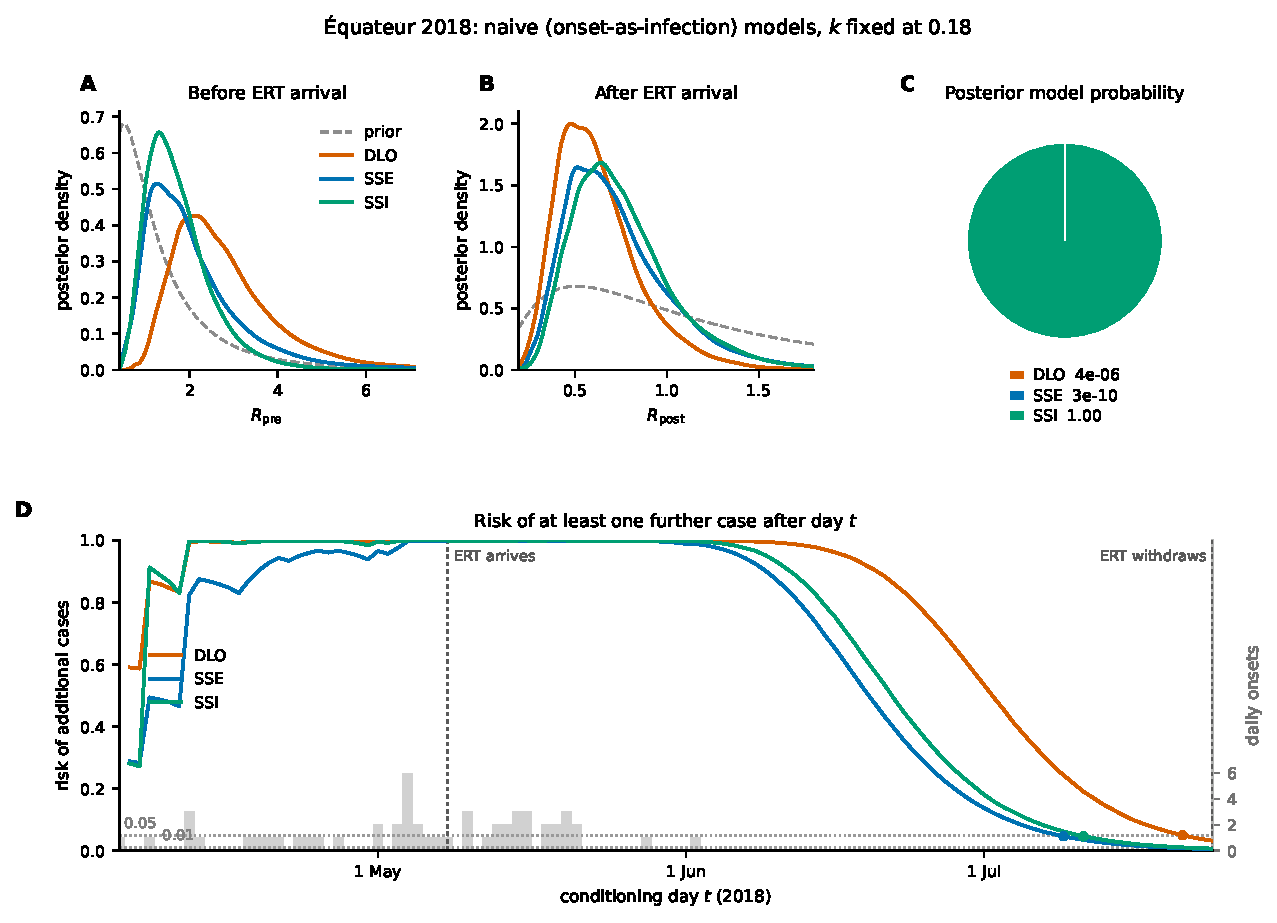
\includegraphics[width=\textwidth]{../figures/naive_models_fixed_k/naive_models_fixed_k.pdf}
  \caption{\textbf{The mechanism of overdispersion changes the end-of-outbreak risk, at a
    dispersion parameter that is only meaningful for two of the three models.} \dlo{}, \sse{}
    and \ssi{} fitted to the \'Equateur onset series with $k$ fixed at
    \resultnum{naivemodelsfixedk.fixedk}. \textbf{A}, \textbf{B}: posterior densities for
    $\Rpre$ and $\Rpost$, over the shared prior. \textbf{C}: posterior model probabilities under
    a uniform prior over the \resultnum{naivemodelsfixedk.nmodels} models; one of the three is
    deliberately miscalibrated, so this panel is evidence about the models \emph{as specified},
    priors included. \textbf{D}: risk of additional cases against conditioning day, with daily
    onsets behind it, the ERT arrival and withdrawal marked, and the $0.05$ and $0.01$ decision
    thresholds drawn. The marker on each curve is its $0.05$ crossing.}
  \label{fig:naive-fixed}
\end{figure}

\begin{itemize}
  \item \textbf{The same $k$ buys \dlo{} almost no overdispersion.} At
    day~\resultnum{data.referenceday} the risk is
    \resultnum{naivemodelsfixedk.dlo.rac.reference} under \dlo{} against
    \resultnum{naivemodelsfixedk.sse.rac.reference} under \sse{} and
    \resultnum{naivemodelsfixedk.ssi.rac.reference} under \ssi{} --- a factor of more than four
    between models handed an identical dispersion parameter. This is the dilution bound
    \eqref{eq:dlo-bounds} in practice: the future force of infection after the last case is thin
    and spread over the whole serial interval, which is exactly the regime in which a day-level
    $k$ does almost nothing and \dlo{} is pressed against its Poisson lower bound.
  \item \textbf{The consequence for a declaration is weeks, not days.} \dlo{}'s risk first
    settles below $0.05$ on day~\resultnum{naivemodelsfixedk.dlo.rac05.day}
    (\resultnum{naivemodelsfixedk.dlo.rac05.date}), against
    day~\resultnum{naivemodelsfixedk.sse.rac05.day} for \sse{} and
    day~\resultnum{naivemodelsfixedk.ssi.rac05.day} for \ssi{}. At the $0.01$ threshold \dlo{}
    \textbf{\resultnum{naivemodelsfixedk.dlo.rac01.day}} settles within the analysis window,
    while \sse{} does so on day~\resultnum{naivemodelsfixedk.sse.rac01.day} and \ssi{} on
    day~\resultnum{naivemodelsfixedk.ssi.rac01.day}. On the day the ERT actually withdrew,
    \dlo{} still places \resultnum{naivemodelsfixedk.dlo.rac.final} on a further case, against
    \resultnum{naivemodelsfixedk.sse.rac.final} and \resultnum{naivemodelsfixedk.ssi.rac.final}.
  \item \textbf{\ssi{} lies on the same side of \sse{} as \dlo{} does.} After the final case
    \ssi{}'s risk is \emph{above} \sse{}'s
    (\resultnum{naivemodelsfixedk.ssi.rac.reference} against
    \resultnum{naivemodelsfixedk.sse.rac.reference} at day~\resultnum{data.referenceday}), which
    reads backwards until one asks what each model's heterogeneity is attached to. \ssi{}'s is a
    property of \emph{people who have been observed}: \resultnum{data.totalcases} known
    individuals have now gone weeks without infecting anyone, which is direct evidence they were
    not the superspreading kind, and $\Lambda_Y(t)$ is revised down accordingly. \sse{}'s is a
    property of \emph{events that have not happened yet}, about which a run of zeros says
    nothing, so \sse{} gets no such revision --- its entire retained state is $\Lambda(t)$. At
    matched expected further cases, \sse{}'s residual risk is a rare burst and \ssi{}'s a more
    likely singleton, and the question ``any further case?'' sees the second as the larger risk.
    So the axis is not naive-versus-mechanistic: it is how many units the same $\Lambda(t)$ is
    divided over and whether each unit's dispersion survives to time $t$. \dlo{} divides over
    future days, \ssi{} over past individuals, \sse{} not at all.
  \item \textbf{The ordering is a property of the question as much as of the models.} Asking
    instead whether transmission would re-establish reverses \sse{} and \ssi{} on these same
    data, because a cluster seeds a new chain far more readily than a lone case. Both orderings
    are correct answers to different questions, and the end-of-outbreak criterion in use asks the
    first.
  \item \textbf{The model probabilities strongly favour \ssi{}} ---
    \resultnum{naivemodelsfixedk.ssi.probability} against
    \resultnum{naivemodelsfixedk.dlo.probability} for \dlo{} and
    \resultnum{naivemodelsfixedk.sse.probability} for \sse{}, from log evidences of
    \resultnum{naivemodelsfixedk.ssi.logevidence}, \resultnum{naivemodelsfixedk.dlo.logevidence}
    and \resultnum{naivemodelsfixedk.sse.logevidence} nats. At a fixed $k$ this partly reports
    that \resultnum{naivemodelsfixedk.fixedk} is a better value for \ssi{} than for the other
    two, which is the transplantation error restated rather than independent evidence about
    mechanism. Analysis~2 separates the two readings.
  \item \textbf{$\Rpost$ is comparable across the three models} ---
    \resultnum{naivemodelsfixedk.dlo.rpost.interval},
    \resultnum{naivemodelsfixedk.sse.rpost.interval} and
    \resultnum{naivemodelsfixedk.ssi.rpost.interval} (posterior median and 95\% credible
    interval) --- so the divergence in the risk curves does not come from a different inferred
    effect of the intervention. The corresponding $\Rpre$ estimates are
    \resultnum{naivemodelsfixedk.dlo.rpre.interval},
    \resultnum{naivemodelsfixedk.sse.rpre.interval} and
    \resultnum{naivemodelsfixedk.ssi.rpre.interval}.
  \item \textbf{Monte-Carlo error does not account for the separation.} Over the case-free tail
    in which the crossings occur, the largest Monte-Carlo standard error on any of the three
    curves is \resultnum{naivemodelsfixedk.ssi.rac.mcselate}, two orders of magnitude below the
    differences above.
\end{itemize}

% ---------------------------------------------------------------------------------------------
\subsection{Mechanism, with the dispersion estimated}
\label{sec:results-naive-estimated}

\begin{figure}[htbp]
  \centering
  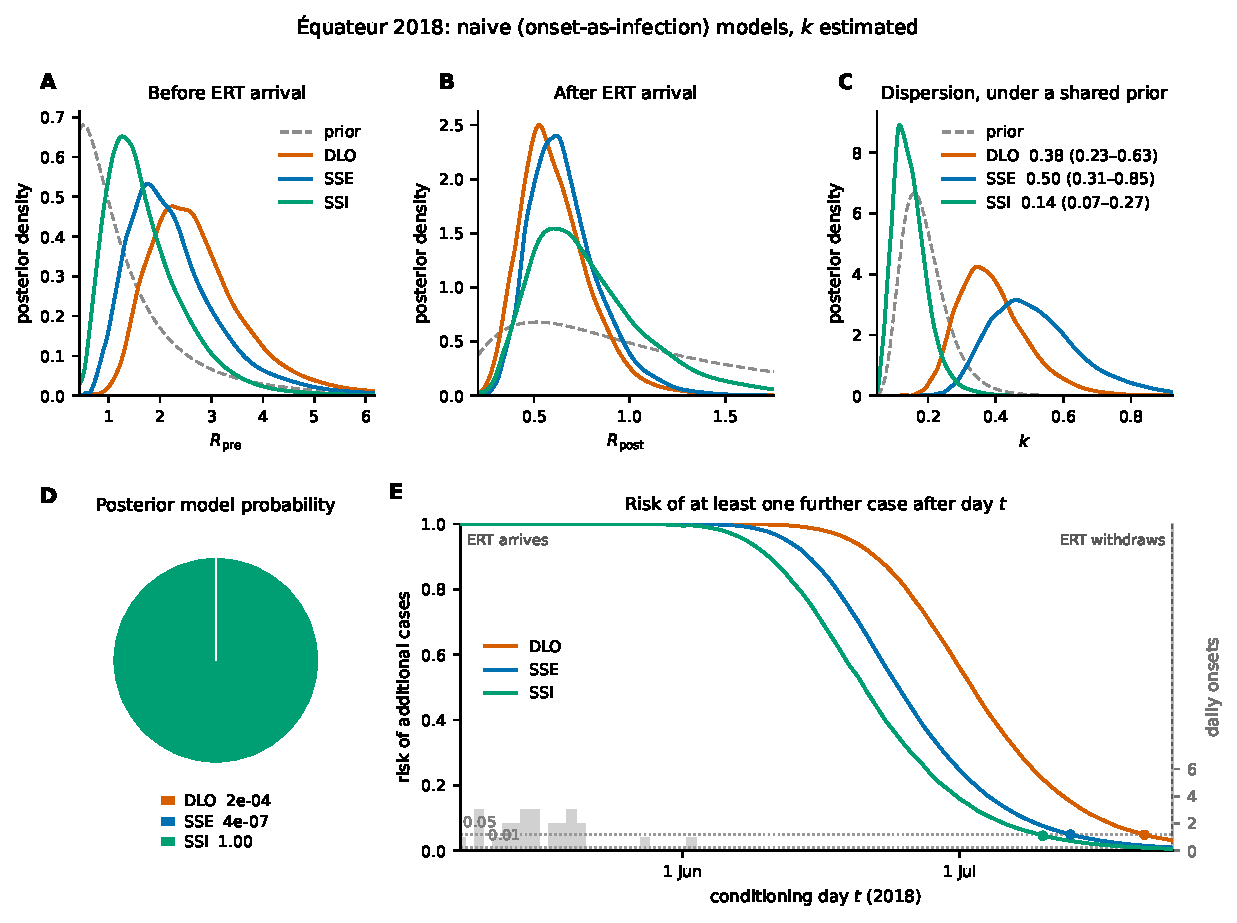
\includegraphics[width=\textwidth]{../figures/naive_models_estimated_k/naive_models_estimated_k.pdf}
  \caption{\textbf{Estimating $k$ under a shared prior shows that the models want different
    values of it --- and that the risk gap survives anyway.} As Fig.~\ref{fig:naive-fixed}, with
    $k$ estimated. \textbf{C}: the three $k$ posteriors over the prior they share, with each
    model's posterior median and 95\% credible interval in the legend. \textbf{D}: posterior
    model probabilities. \textbf{E}: risk of additional cases, with the view starting at the
    ERT's arrival because all three curves sit flat at $1$ until well past the last case.}
  \label{fig:naive-estimated}
\end{figure}

\begin{itemize}
  \item \textbf{The models disagree about $k$, but not along the axis one might expect.} The
    posterior medians (95\% credible intervals) are
    \resultnum{naivemodelsestimatedk.dlo.k.interval} for \dlo{},
    \resultnum{naivemodelsestimatedk.sse.k.interval} for \sse{} and
    \resultnum{naivemodelsestimatedk.ssi.k.interval} for \ssi{}. \dlo{} against \ssi{}: overlap
    \resultnum{naivemodelsestimatedk.dlo-vs-ssi.overlap}, median ratio
    \resultnum{naivemodelsestimatedk.dlo-vs-ssi.medianratio},
    $\Pr(k_{\mdlo}>k_{\mssi})=\resultnum{naivemodelsestimatedk.dlo-vs-ssi.probabilitygreater}$.
    \sse{} against \ssi{}: overlap \resultnum{naivemodelsestimatedk.sse-vs-ssi.overlap}, ratio
    \resultnum{naivemodelsestimatedk.sse-vs-ssi.medianratio}, probability
    \resultnum{naivemodelsestimatedk.sse-vs-ssi.probabilitygreater}. But \dlo{} against \sse{}:
    overlap \resultnum{naivemodelsestimatedk.dlo-vs-sse.overlap} and
    $\Pr(k_{\mdlo}>k_{\msse})=\resultnum{naivemodelsestimatedk.dlo-vs-sse.probabilitygreater}$ ---
    the two are barely distinguishable. \textbf{It is \ssi{} that is the outlier, not \dlo{}.}
  \item \textbf{The split is day-level against individual-level, which is where
    onset-as-infection bites hardest.} \dlo{} and \sse{} both attach their excess variance to a
    \emph{day}: \dlo{} to the day's aggregate incidence, \sse{} to the day's pooled transmission
    through a freshly drawn $\lambda_t$. \ssi{} attaches it to the \emph{individual}. The series
    being fitted is onsets, and an incubation period of mean \resultnum{delays.incubation.mean}\,d
    and standard deviation \resultnum{delays.incubation.sd}\,d scatters each day's infections
    forward over a wide kernel --- so a model reading onsets as infections sees day-to-day
    variation that the convolution has already largely averaged out, and answers with a larger
    $k$ (less overdispersion) than the infection process carried. \ssi{} is close to invariant to
    this, because the convolution \emph{regroups} individuals across days while the aggregate
    infectivity of $n$ independent individuals is $\Gam(kn,k)$ whichever $n$ they are: regrouping
    moves the cohorts, not the variance. This is a proposed mechanism for the measurement, not a
    second measurement --- these three models are all infection-anchored, so this analysis cannot
    separate it from the purely structural difference of Section~\ref{sec:structure}.
    Section~\ref{sec:results-onset} is where it is tested.
  \item \textbf{Only \ssi{}'s posterior is compatible with the literature value.} \ssi{}'s 95\%
    credible interval, $(\resultnum{naivemodelsestimatedk.ssi.k.lower},
    \resultnum{naivemodelsestimatedk.ssi.k.upper})$, contains
    \resultnum{naivemodelsfixedk.fixedk}; \dlo{}'s
    $(\resultnum{naivemodelsestimatedk.dlo.k.lower},
    \resultnum{naivemodelsestimatedk.dlo.k.upper})$ and \sse{}'s
    $(\resultnum{naivemodelsestimatedk.sse.k.lower},
    \resultnum{naivemodelsestimatedk.sse.k.upper})$ do not, and both medians sit above the
    prior's own 97.5th percentile of \resultnum{priors.k.quantileupper}, despite that prior being
    deliberately informative.
  \item \textbf{The evidence says the same thing more sharply.} Letting $k$ move is worth
    \resultnum{naivemodelsestimatedk.sse.evidencegain} nats to \sse{} and
    \resultnum{naivemodelsestimatedk.dlo.evidencegain} to \dlo{}, but only
    \resultnum{naivemodelsestimatedk.ssi.evidencegain} to \ssi{}. Analysis~1 was charging \dlo{}
    and \sse{} for a value that was never theirs, and \resultnum{naivemodelsfixedk.fixedk} really
    is \ssi{}'s number on this series.
  \item \textbf{The risk gap survives, which is the point of the pairing.} Each model now sits at
    its own best $k$, and \dlo{} still crosses $0.05$ on
    day~\resultnum{naivemodelsestimatedk.dlo.rac05.day}, against
    day~\resultnum{naivemodelsestimatedk.sse.rac05.day} for \sse{} and
    day~\resultnum{naivemodelsestimatedk.ssi.rac05.day} for \ssi{}, and still
    \textbf{\resultnum{naivemodelsestimatedk.dlo.rac01.day}} reaches $0.01$ inside the window,
    where \sse{} does on day~\resultnum{naivemodelsestimatedk.sse.rac01.day} and \ssi{} on
    day~\resultnum{naivemodelsestimatedk.ssi.rac01.day}. Misapplying a literature $k$ creates the
    gap; the day-level mechanism sustains it.
  \item \textbf{The posterior model probabilities keep their direction} --- \ssi{}
    \resultnum{naivemodelsestimatedk.ssi.probability}, \dlo{}
    \resultnum{naivemodelsestimatedk.dlo.probability}, \sse{}
    \resultnum{naivemodelsestimatedk.sse.probability} --- and now carry a cleaner reading, since
    each model has been allowed its own dispersion.
\end{itemize}

% ---------------------------------------------------------------------------------------------
\subsection{Onset anchoring}
\label{sec:results-onset}

\begin{figure}[htbp]
  \centering
  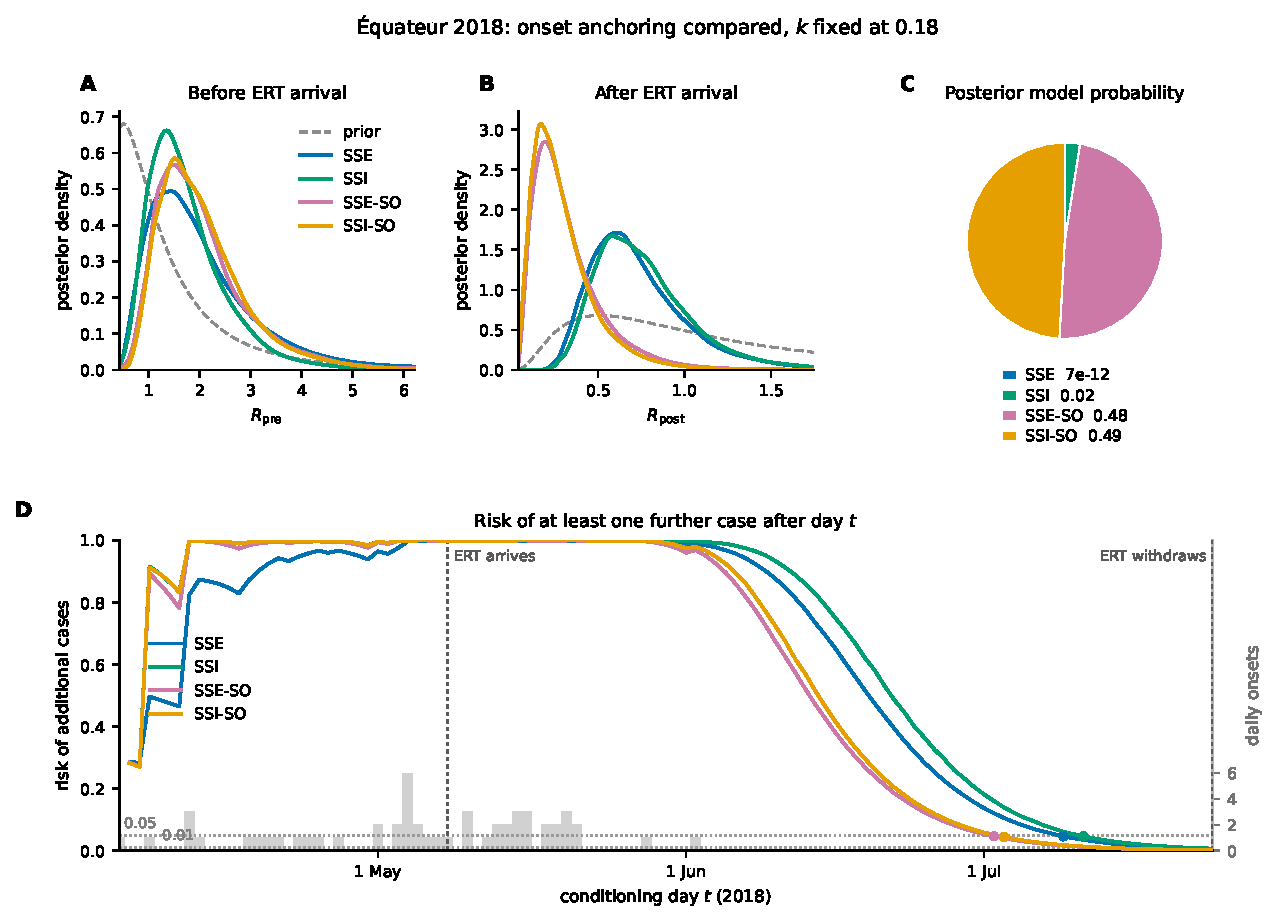
\includegraphics[width=\textwidth]{../figures/onset_models_fixed_k/onset_models_fixed_k.pdf}
  \caption{\textbf{Onset anchoring at a fixed dispersion parameter.} \sse{}, \ssi{}, \sseso{} and
    \ssiso{} with $k$ held at \resultnum{onsetmodelsfixedk.fixedk}; panels as in
    Fig.~\ref{fig:naive-fixed}, with a uniform prior over
    \resultnum{onsetmodelsfixedk.nmodels} models in \textbf{C}. All four models are driven by the
    same onset-to-onset serial interval, so the comparison isolates anchoring.}
  \label{fig:onset-fixed}
\end{figure}

\begin{figure}[htbp]
  \centering
  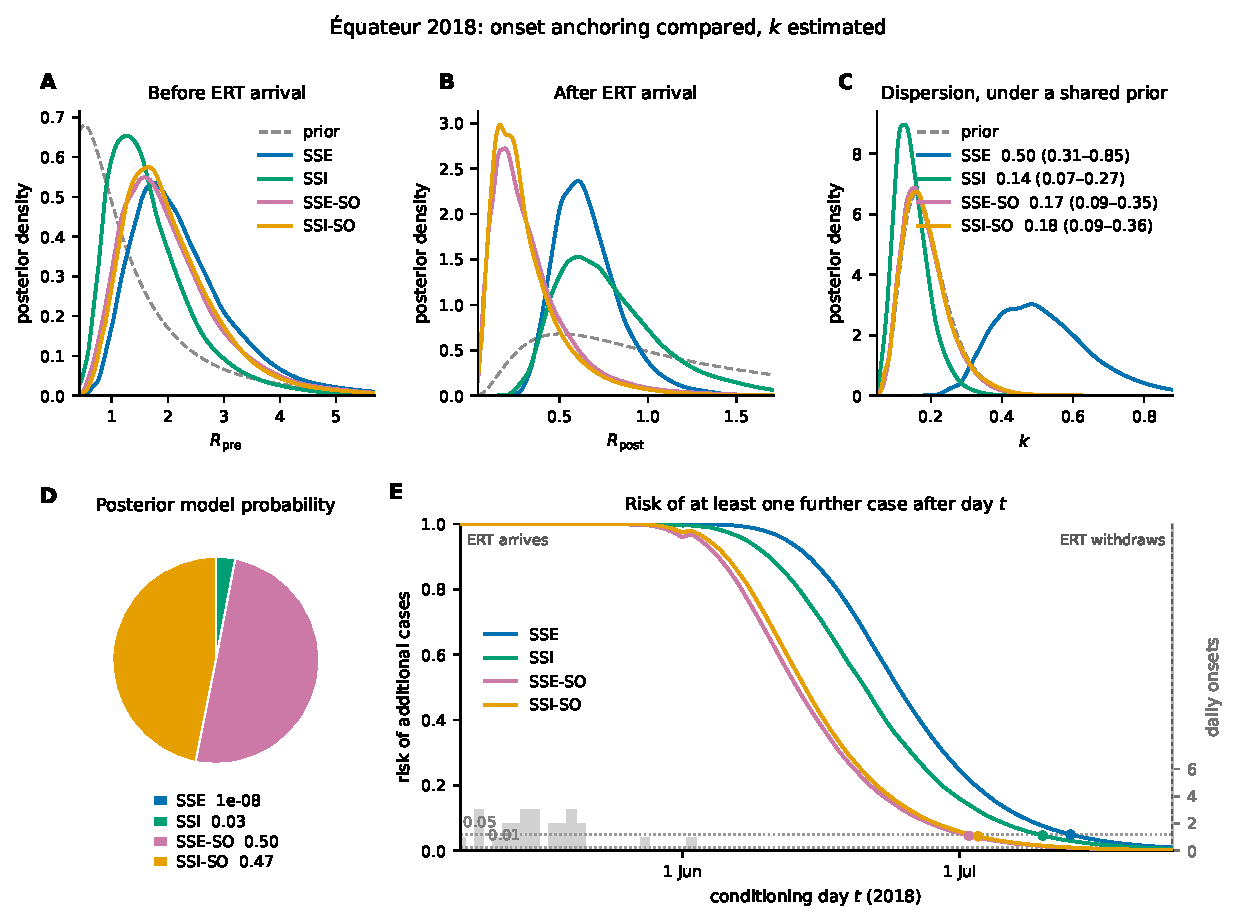
\includegraphics[width=\textwidth]{../figures/onset_models_estimated_k/onset_models_estimated_k.pdf}
  \caption{\textbf{Onset anchoring with the dispersion estimated.} Panels as in
    Fig.~\ref{fig:naive-estimated}. Panel~\textbf{C} is where the attenuation hypothesis of
    Section~\ref{sec:results-naive-estimated} is settled: \sseso{}'s $k$ posterior should sit
    below naive \sse{}'s if incubation convolution is what inflates day-level dispersion
    estimates, while \ssiso{}'s should barely move from \ssi{}'s.}
  \label{fig:onset-estimated}
\end{figure}

\begin{itemize}
  \item \textbf{Onset anchoring advances both crossings by 8--12 days.} With $k$ estimated
    (Fig.~\ref{fig:onset-estimated}), \sseso{} crosses $0.05$ on
    day~\resultnum{onsetmodelsestimatedk.sseso.rac05.day} against \sse{}'s
    day~\resultnum{onsetmodelsestimatedk.sse.rac05.day}, an advance of
    \resultnum{onsetmodelsestimatedk.sseso-vs-sse.shift05} days, and $0.01$ on
    day~\resultnum{onsetmodelsestimatedk.sseso.rac01.day} against
    day~\resultnum{onsetmodelsestimatedk.sse.rac01.day}, an advance of
    \resultnum{onsetmodelsestimatedk.sseso-vs-sse.shift01} days. \ssiso{} advances \ssi{}'s
    crossings by \resultnum{onsetmodelsestimatedk.ssiso-vs-ssi.shift05} and
    \resultnum{onsetmodelsestimatedk.ssiso-vs-ssi.shift01} days respectively
    (day~\resultnum{onsetmodelsestimatedk.ssiso.rac05.day} against
    day~\resultnum{onsetmodelsestimatedk.ssi.rac05.day}, and
    day~\resultnum{onsetmodelsestimatedk.ssiso.rac01.day} against
    day~\resultnum{onsetmodelsestimatedk.ssi.rac01.day}). At a fixed $k$
    (Fig.~\ref{fig:onset-fixed}) the same comparisons give
    \resultnum{onsetmodelsfixedk.sseso-vs-sse.shift05} and
    \resultnum{onsetmodelsfixedk.sseso-vs-sse.shift01} days for \sseso{} against \sse{}, and
    \resultnum{onsetmodelsfixedk.ssiso-vs-ssi.shift05} and
    \resultnum{onsetmodelsfixedk.ssiso-vs-ssi.shift01} days for \ssiso{} against \ssi{}. The
    displacement is on the scale of the mean incubation period,
    \resultnum{delays.incubation.mean}\,d.
  \item \textbf{Why the direction is \emph{earlier}, and why it is not a shorter generation
    time.} All four models share the same onset-to-onset serial interval; what changes is which
    side of the conditioning day a transmission falls on once that interval is cut into
    transmission and incubation pieces. Proposition~\ref{prop:onset} makes this explicit: the
    onset-anchored models place infection at transmission time, so infections already generated
    under the historical $\Rpost$ enter $M(t)$ and stay in the incubation pipeline when control is
    reset, while the remaining TOST opportunity $W(t)$ of older onset cohorts is already largely
    spent. The infection-anchored models have no pipeline, move the infection decision to the
    later symptom-onset date, and apply the reset $\Rreset$ to it, which makes the residual state
    look younger and drain later.
  \item \textbf{The same indexing error inflates the naive $\Rpost$ roughly threefold.} With $k$
    estimated the posterior medians (95\% credible intervals) are
    \resultnum{onsetmodelsestimatedk.sse.rpost.interval} for \sse{} and
    \resultnum{onsetmodelsestimatedk.ssi.rpost.interval} for \ssi{}, against
    \resultnum{onsetmodelsestimatedk.sseso.rpost.interval} for \sseso{} and
    \resultnum{onsetmodelsestimatedk.ssiso.rpost.interval} for \ssiso{}. The naive convention
    applies the day-\resultnum{data.ertarrivalday} switch to \emph{onsets}, so post-arrival onsets
    that arose from pre-arrival infections are charged to the controlled period. $\Rpre$ is far
    more stable across the four --- \resultnum{onsetmodelsestimatedk.sse.rpre.interval},
    \resultnum{onsetmodelsestimatedk.ssi.rpre.interval},
    \resultnum{onsetmodelsestimatedk.sseso.rpre.interval} and
    \resultnum{onsetmodelsestimatedk.ssiso.rpre.interval} --- which is what one expects if the
    effect concerns \emph{when} the switch lands rather than the epidemic's early growth.
  \item \textbf{The attenuation hypothesis passes.} \sseso{}'s $k$ posterior,
    \resultnum{onsetmodelsestimatedk.sseso.k.interval}, sits below naive \sse{}'s
    \resultnum{onsetmodelsestimatedk.sse.k.interval} and towards the literature value: median
    ratio \resultnum{onsetmodelsestimatedk.sse-vs-sseso.medianratio}, overlap
    \resultnum{onsetmodelsestimatedk.sse-vs-sseso.overlap},
    $\Pr(k_{\msse}>k_{\msseso}) =
     \resultnum{onsetmodelsestimatedk.sse-vs-sseso.probabilitygreater}$. \ssi{} moves far less ---
    \resultnum{onsetmodelsestimatedk.ssi.k.interval} against \ssiso{}'s
    \resultnum{onsetmodelsestimatedk.ssiso.k.interval}, overlap
    \resultnum{onsetmodelsestimatedk.ssi-vs-ssiso.overlap}. Incubation convolution attenuates
    \emph{day-level} dispersion when onsets are read as infections; individual-level dispersion is
    comparatively stable under regrouping, as predicted.
  \item \textbf{Once anchoring is explicit, the mechanism stops mattering for $k$.} \sseso{} and
    \ssiso{} agree almost exactly --- overlap
    \resultnum{onsetmodelsestimatedk.sseso-vs-ssiso.overlap}, median ratio
    \resultnum{onsetmodelsestimatedk.sseso-vs-ssiso.medianratio},
    $\Pr(k_{\msseso}>k_{\mssiso}) =
     \resultnum{onsetmodelsestimatedk.sseso-vs-ssiso.probabilitygreater}$ --- where their naive
    counterparts differ by a factor of
    \resultnum{onsetmodelsestimatedk.sse-vs-ssi.medianratio} at an overlap of
    \resultnum{onsetmodelsestimatedk.sse-vs-ssi.overlap}. The event-versus-individual gap of
    Section~\ref{sec:results-naive-estimated} was to a large extent the conflation, not the
    mechanism.
  \item \textbf{The onset-anchored models are strongly preferred, and are indistinguishable from
    each other.} With $k$ estimated the posterior model probabilities are
    \resultnum{onsetmodelsestimatedk.sseso.probability} for \sseso{} and
    \resultnum{onsetmodelsestimatedk.ssiso.probability} for \ssiso{}, against
    \resultnum{onsetmodelsestimatedk.ssi.probability} for \ssi{} and
    \resultnum{onsetmodelsestimatedk.sse.probability} for \sse{}; the log evidences are
    \resultnum{onsetmodelsestimatedk.sseso.logevidence},
    \resultnum{onsetmodelsestimatedk.ssiso.logevidence},
    \resultnum{onsetmodelsestimatedk.ssi.logevidence} and
    \resultnum{onsetmodelsestimatedk.sse.logevidence} nats. The fixed-$k$ analysis gives the same
    ordering (\resultnum{onsetmodelsfixedk.sseso.probability},
    \resultnum{onsetmodelsfixedk.ssiso.probability},
    \resultnum{onsetmodelsfixedk.ssi.probability},
    \resultnum{onsetmodelsfixedk.sse.probability}).
  \item \textbf{The onset-anchored models gain nothing from estimating $k$, which is a
    consistency check on the two preceding points.} Releasing $k$ is worth
    \resultnum{onsetmodelsestimatedk.sseso.evidencegain} nats to \sseso{} and
    \resultnum{onsetmodelsestimatedk.ssiso.evidencegain} to \ssiso{} --- within their own
    estimation error --- against \resultnum{onsetmodelsestimatedk.sse.evidencegain} for naive
    \sse{}. Their $k$ posteriors already sit on \resultnum{onsetmodelsfixedk.fixedk}, so fixing it
    there costs them nothing.
  \item \textbf{The direction of the 8--12-day advance should not be universalised.} It is
    measured under this reset convention, this switch convention, this outbreak history and this
    posterior. The incubation-scale explanation is the mechanism for \emph{this} result, not a
    theorem for arbitrary time series or interventions.
\end{itemize}

\begin{table}[htbp]
  \centering
  \caption{Threshold crossings of the risk of additional cases across the four analyses: the
    first day on which the curve settles below the threshold, with the calendar date. The ERT
    withdrew on day~\resultnum{data.withdrawalday} (\resultnum{data.withdrawaldate});
    ``never'' means the curve had not settled below the threshold by then.}
  \label{tab:crossings}
  \small
  \begin{tabular}{llcccc}
    \toprule
    Analysis & Model & \multicolumn{2}{c}{$\RAC < 0.05$} & \multicolumn{2}{c}{$\RAC < 0.01$} \\
    \cmidrule(lr){3-4}\cmidrule(lr){5-6}
    & & day & date & day & date \\
    \midrule
    1: naive, $k=\resultnum{naivemodelsfixedk.fixedk}$
      & \dlo{}   & \resultnum{naivemodelsfixedk.dlo.rac05.day}   & \resultnum{naivemodelsfixedk.dlo.rac05.date}
                 & \resultnum{naivemodelsfixedk.dlo.rac01.day}   & \resultnum{naivemodelsfixedk.dlo.rac01.date} \\
      & \sse{}   & \resultnum{naivemodelsfixedk.sse.rac05.day}   & \resultnum{naivemodelsfixedk.sse.rac05.date}
                 & \resultnum{naivemodelsfixedk.sse.rac01.day}   & \resultnum{naivemodelsfixedk.sse.rac01.date} \\
      & \ssi{}   & \resultnum{naivemodelsfixedk.ssi.rac05.day}   & \resultnum{naivemodelsfixedk.ssi.rac05.date}
                 & \resultnum{naivemodelsfixedk.ssi.rac01.day}   & \resultnum{naivemodelsfixedk.ssi.rac01.date} \\
    \addlinespace
    2: naive, $k$ estimated
      & \dlo{}   & \resultnum{naivemodelsestimatedk.dlo.rac05.day}   & \resultnum{naivemodelsestimatedk.dlo.rac05.date}
                 & \resultnum{naivemodelsestimatedk.dlo.rac01.day}   & \resultnum{naivemodelsestimatedk.dlo.rac01.date} \\
      & \sse{}   & \resultnum{naivemodelsestimatedk.sse.rac05.day}   & \resultnum{naivemodelsestimatedk.sse.rac05.date}
                 & \resultnum{naivemodelsestimatedk.sse.rac01.day}   & \resultnum{naivemodelsestimatedk.sse.rac01.date} \\
      & \ssi{}   & \resultnum{naivemodelsestimatedk.ssi.rac05.day}   & \resultnum{naivemodelsestimatedk.ssi.rac05.date}
                 & \resultnum{naivemodelsestimatedk.ssi.rac01.day}   & \resultnum{naivemodelsestimatedk.ssi.rac01.date} \\
    \addlinespace
    3: onset, $k=\resultnum{onsetmodelsfixedk.fixedk}$
      & \sse{}   & \resultnum{onsetmodelsfixedk.sse.rac05.day}   & \resultnum{onsetmodelsfixedk.sse.rac05.date}
                 & \resultnum{onsetmodelsfixedk.sse.rac01.day}   & \resultnum{onsetmodelsfixedk.sse.rac01.date} \\
      & \ssi{}   & \resultnum{onsetmodelsfixedk.ssi.rac05.day}   & \resultnum{onsetmodelsfixedk.ssi.rac05.date}
                 & \resultnum{onsetmodelsfixedk.ssi.rac01.day}   & \resultnum{onsetmodelsfixedk.ssi.rac01.date} \\
      & \sseso{} & \resultnum{onsetmodelsfixedk.sseso.rac05.day} & \resultnum{onsetmodelsfixedk.sseso.rac05.date}
                 & \resultnum{onsetmodelsfixedk.sseso.rac01.day} & \resultnum{onsetmodelsfixedk.sseso.rac01.date} \\
      & \ssiso{} & \resultnum{onsetmodelsfixedk.ssiso.rac05.day} & \resultnum{onsetmodelsfixedk.ssiso.rac05.date}
                 & \resultnum{onsetmodelsfixedk.ssiso.rac01.day} & \resultnum{onsetmodelsfixedk.ssiso.rac01.date} \\
    \addlinespace
    4: onset, $k$ estimated
      & \sse{}   & \resultnum{onsetmodelsestimatedk.sse.rac05.day}   & \resultnum{onsetmodelsestimatedk.sse.rac05.date}
                 & \resultnum{onsetmodelsestimatedk.sse.rac01.day}   & \resultnum{onsetmodelsestimatedk.sse.rac01.date} \\
      & \ssi{}   & \resultnum{onsetmodelsestimatedk.ssi.rac05.day}   & \resultnum{onsetmodelsestimatedk.ssi.rac05.date}
                 & \resultnum{onsetmodelsestimatedk.ssi.rac01.day}   & \resultnum{onsetmodelsestimatedk.ssi.rac01.date} \\
      & \sseso{} & \resultnum{onsetmodelsestimatedk.sseso.rac05.day} & \resultnum{onsetmodelsestimatedk.sseso.rac05.date}
                 & \resultnum{onsetmodelsestimatedk.sseso.rac01.day} & \resultnum{onsetmodelsestimatedk.sseso.rac01.date} \\
      & \ssiso{} & \resultnum{onsetmodelsestimatedk.ssiso.rac05.day} & \resultnum{onsetmodelsestimatedk.ssiso.rac05.date}
                 & \resultnum{onsetmodelsestimatedk.ssiso.rac01.day} & \resultnum{onsetmodelsestimatedk.ssiso.rac01.date} \\
    \bottomrule
  \end{tabular}
\end{table}

% ---------------------------------------------------------------------------------------------
\subsection{Cases against transmission: the incubation pipeline}
\label{sec:results-rat}

\begin{figure}[htbp]
  \centering
  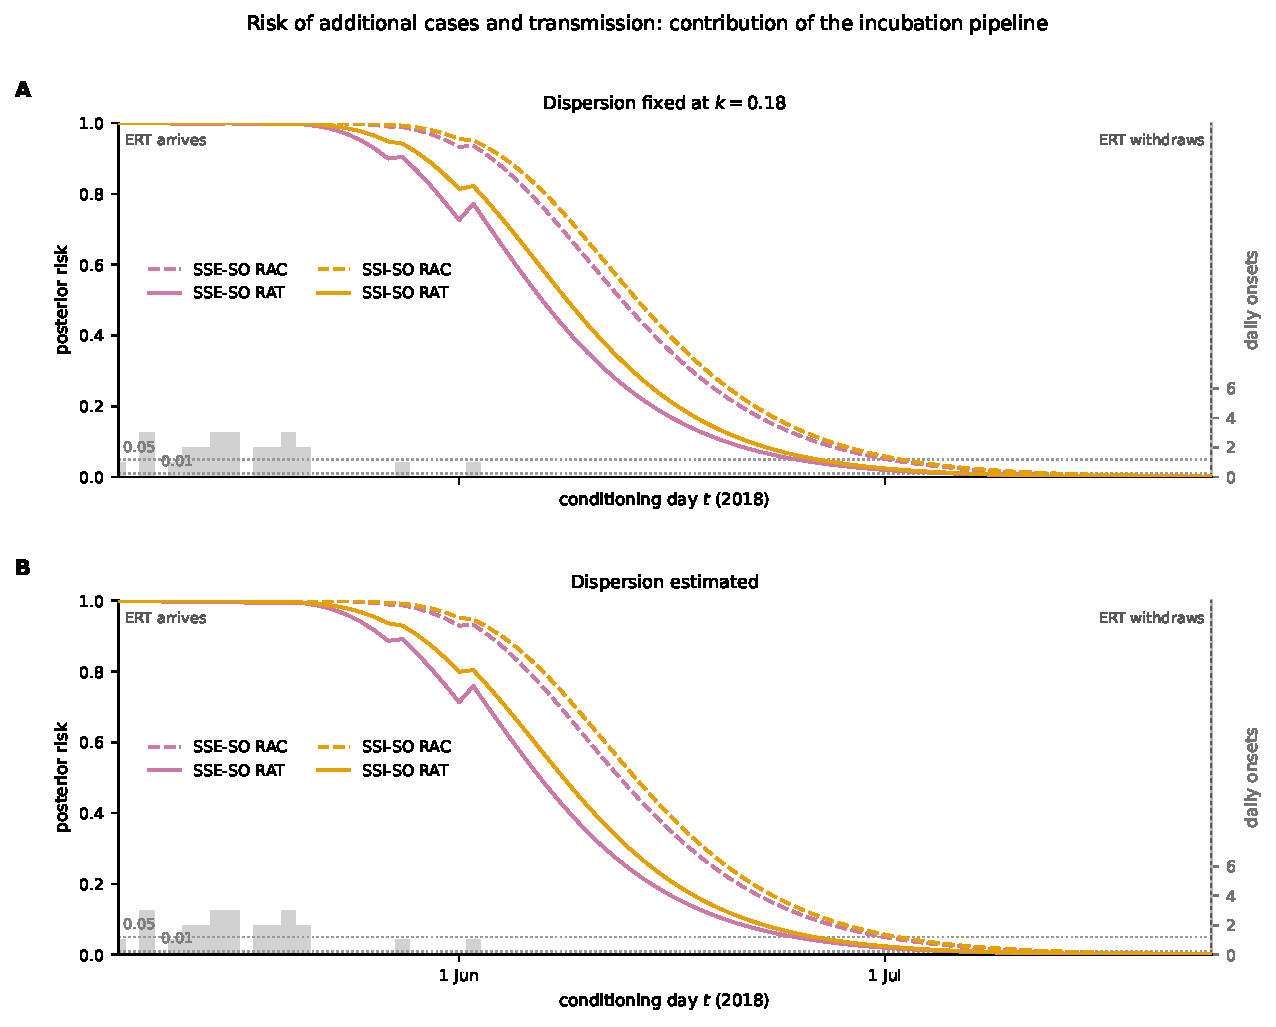
\includegraphics[width=\textwidth]{../figures/onset_models_rat/onset_models_rat.pdf}
  \caption{\textbf{The gap between the risk of additional cases and the risk of additional
    transmission is the incubation pipeline, quantified.} \sseso{} and \ssiso{} with $k$ fixed
    at \resultnum{onsetmodelsfixedk.fixedk} (\textbf{A}) and estimated (\textbf{B}). Dashed:
    $\RAC$. Solid: $\RAT$. The shaded region between them is the $M(t)e^{-c}$ term of
    Proposition~\ref{prop:onset} --- individuals already infected on the conditioning day but not
    yet symptomatic. Under the three infection-anchored models these two curves coincide by
    assumption, which is the conflation being measured.}
  \label{fig:rat}
\end{figure}

\begin{itemize}
  \item \textbf{The pipeline is worth about a quarter of a unit of probability at its widest.}
    With $k$ estimated, $\RAC$ exceeds $\RAT$ by at most
    \resultnum{onsetmodelsestimatedk.sseso.gap.max} for \sseso{}, on
    day~\resultnum{onsetmodelsestimatedk.sseso.gap.day}
    (\resultnum{onsetmodelsestimatedk.sseso.gap.date}), and by at most
    \resultnum{onsetmodelsestimatedk.ssiso.gap.max} for \ssiso{}, on
    day~\resultnum{onsetmodelsestimatedk.ssiso.gap.day}. The gap peaks shortly after the last
    observed onset (day~\resultnum{data.lastonsetday}), when the pipeline is largest relative to
    the transmission still to come, and closes as it drains.
  \item \textbf{It delays a case-based declaration by most of a week.} With $k$ estimated,
    \sseso{}'s $\RAT$ settles below $0.05$ on
    day~\resultnum{onsetmodelsestimatedk.sseso.rat05.day} and below $0.01$ on
    day~\resultnum{onsetmodelsestimatedk.sseso.rat01.day}, against
    day~\resultnum{onsetmodelsestimatedk.sseso.rac05.day} and
    day~\resultnum{onsetmodelsestimatedk.sseso.rac01.day} for $\RAC$ --- later by
    \resultnum{onsetmodelsestimatedk.sseso.gap.shift05} and
    \resultnum{onsetmodelsestimatedk.sseso.gap.shift01} days. For \ssiso{} the same comparison
    gives \resultnum{onsetmodelsestimatedk.ssiso.gap.shift05} and
    \resultnum{onsetmodelsestimatedk.ssiso.gap.shift01} days ($\RAT$ on days
    \resultnum{onsetmodelsestimatedk.ssiso.rat05.day} and
    \resultnum{onsetmodelsestimatedk.ssiso.rat01.day} against $\RAC$ on days
    \resultnum{onsetmodelsestimatedk.ssiso.rac05.day} and
    \resultnum{onsetmodelsestimatedk.ssiso.rac01.day}).
  \item \textbf{The two quantities answer different questions, and the difference is
    decision-relevant.} $\RAT$ isolates what relaxing interventions does; $\RAC$ is what a
    surveillance system would actually see. A criterion written on cases keeps interventions in
    place while the pipeline drains, even though transmission risk has already settled --- and an
    infection-anchored model, which identifies the two by assumption, cannot represent that
    distinction at all.
  \item \textbf{Fixing $k$ changes very little here}, as the near-identical panels show: the
    widest gap is \resultnum{onsetmodelsfixedk.sseso.gap.max} for \sseso{} and
    \resultnum{onsetmodelsfixedk.ssiso.gap.max} for \ssiso{}, against
    \resultnum{onsetmodelsestimatedk.sseso.gap.max} and
    \resultnum{onsetmodelsestimatedk.ssiso.gap.max} when it is estimated --- a consequence of the
    onset-anchored $k$ posteriors already sitting on the literature value.
\end{itemize}

% =============================================================================================
\section{Sensitivity analyses}
\label{sec:sensitivity}
% =============================================================================================

None of the following has been run. They are listed in rough order of how much each would add,
with what it would resolve.

\begin{enumerate}
  \item \textbf{Outbreak-specific serial interval} (mean
    \resultnum{delays.alternativeserialinterval.mean}\,d, standard deviation
    \resultnum{delays.alternativeserialinterval.sd}\,d) --- \emph{infection-anchored models
    only}. Its much lighter tail materially lowers the risk after a long case-free period, and it
    is the estimate that should be preferred where outbreak-specific contact-tracing data exist.
    It is structurally inadmissible for the onset-anchored models
    (Section~\ref{sec:serial-interval}), and that incompatibility should be reported rather than
    worked around: it says something about how much structure the incubation/TOST decomposition
    imposes.
  \item \textbf{Incubation/TOST decomposition.} Hold $w$ fixed and re-run \sseso{} and \ssiso{}
    under two or three other published Ebola incubation estimates, taking the matching TOST from
    the variance budget each time. This bounds how much of the onset-anchoring result rests on
    the particular split used here, which the serial interval alone does not identify.
  \item \textbf{Filtering rather than smoothed latents.} Section~\ref{sec:smoothing} reports the
    signed comparison at a fixed parameter vector; repeating it integrated over the parameter
    posterior would turn the stated approximation into a quantified one for all three
    latent-variable models.
  \item \textbf{Shifted $R$-switch for the infection-anchored models.} The onset-anchoring
    comparison confounds model structure with the indexing convention for the intervention.
    Re-running the naive models with the switch moved back by
    $\mathbb{E}[A] = \resultnum{delays.incubation.mean}$ days separates them: any residual
    difference from the onset-anchored models is then attributable to structure rather than to
    indexing.
  \item \textbf{Non-empty initial incubation pipeline} for the onset-anchored models. Seed one or
    two already-infected individuals at day~\resultnum{data.firstday} with residual incubation
    drawn from $\finc$, and measure the effect on $\Rpre$ and on the risk curve. This is the
    sensitivity that matters if the index case is not epidemiologically identified
    (Section~\ref{sec:outbreak}).
  \item \textbf{Prior sensitivity}, in particular for $k$, whose prior is deliberately informative
    and whose role differs between models.
\end{enumerate}

% =============================================================================================
\appendix
\section{The two forms of the onset-anchored models are equivalent}
\label{app:equivalence}
% =============================================================================================

The ``natural'' definition of an onset-anchored model generates latent infection counts and maps
them forward to onsets; the inference-convenient forms of \eqref{eq:coriso}--\eqref{eq:ssiso}
work directly with onsets. They define the same joint law for the observed onset process
$(D_t)$.

In the natural form, with $\lambda_t = \sum_{s\ge0}\ftost_s D_{t-s}$ (\coriso{}, \sseso{}) or
$\lambda_t = \sum_{s\ge0}\ftost_s Y_{t-s}$ (\ssiso{}): (i) infections $J_t$ are drawn from the
model's offspring distribution with mean $R_t\lambda_t$; (ii) the $J_u$ infections of day $u$ are
allocated to onset days by independent incubation draws,
$(N_{u,a})_{a\ge1}\mid J_u \sim \mathrm{Multinomial}(J_u, (\finc_a))$; and (iii) onsets are
$D_t = \sum_{a\ge1} N_{t-a,a}$.

\subsection*{The Poisson case}

Let $E_t = R_t\lambda_t$, so $J_t \mid E_t \sim \Pois(E_t)$.

\emph{Step 1 --- Poisson thinning.} Multinomial splitting of a Poisson count yields
\emph{independent} Poisson parts: conditional on $E_u$, $N_{u,a}\sim\Pois(E_u\finc_a)$
independently over $a \ge 1$, with $J_u = \sum_a N_{u,a}$ recovered as their sum. The latent
$J_u$ therefore carries no information beyond the parts and can be dropped. (This is also the
step that makes the incubation pipeline of \eqref{eq:pipeline} Poisson.)

\emph{Step 2 --- Poisson superposition.} $D_t = \sum_{a\ge1}N_{t-a,a}$ is a sum of independent
Poissons, hence $D_t \mid (E_u)_{u<t} \sim \Pois\bigl(\sum_{a\ge1}\finc_a E_{t-a}\bigr)$, which
is \eqref{eq:onset-step}.

\emph{Step 3 --- the joint law, not just the marginal.} Because $\finc$ has no mass at lag~$0$,
$E_{t-a}$ for $a\ge1$ is a function of $D_{0:t-1}$ only, so the display above is precisely the
conditional law $p(D_t \mid D_{0:t-1})$. The parts $\{N_{u,a} : u+a=t\}$ composing $D_t$ are
disjoint from those composing any other $D_{t'}$, so distinct days' onsets are conditionally
independent given the $E$s. Chaining $p(D_{0:T}) = \prod_t p(D_t\mid D_{0:t-1})$ gives equality
of the full joint laws. \hfill$\square$

\subsection*{\sseso{}}

\emph{Step A --- Poisson--Gamma mixture.} If $\tilde\lambda_t\sim\Gam(k\lambda_t,k)$ and
$J_t\mid\tilde\lambda_t\sim\Pois(R_t\tilde\lambda_t)$, then
$R_t\tilde\lambda_t\sim\Gam(k\lambda_t,\ k/R_t)$ and, marginally,
$J_t\sim\NB(\text{mean}=R_t\lambda_t,\ \text{disp}=k\lambda_t)$, which is the natural-form
offspring law. The inference-convenient form merely \emph{un-marginalises} the negative binomial
into an explicit per-day Gamma random effect.

\emph{Step B.} Conditional on $\tilde\lambda_t$ the infection counts are Poisson, so Steps 1--3
apply verbatim. The $\tilde\lambda_t$ are independent across $t$ given $(\lambda_t)$, and each
$\lambda_t$ is a function of $D_{\le t}$, so the day-$t$ conditional still depends only on
$D_{0:t-1}$ once $\tilde\lambda_{<t}$ is integrated out. \hfill$\square$

\subsection*{\ssiso{}}

Identical to the Poisson case with $E_t = R_t\sum_{s\ge0}\ftost_s Y_{t-s}$. The Gamma
infectivities are already explicit in both forms, and the thinning and superposition arguments do
not touch them. \hfill$\square$

% =============================================================================================
\section{Code and reproducibility}
\label{app:reproducibility}
% =============================================================================================

The analysis is implemented in Python and orchestrated with Snakemake in three tiers --- model
fitting, derived quantities, and figures --- so that a change at one tier does not re-run those
above it. The committed repository contains the padded onset series, every posterior sample,
every derived quantity, all figures and this document; \verb|snakemake| reproduces all of them
from the raw data.

\textbf{No number in this document is typed into the prose.} Each is a macro expanded from a
generated file that a pipeline rule writes from the posterior samples and derived quantities, so
a refit moves the numbers in the text as well as on the figures, and a key with no value is a
compilation error rather than a blank. Quantities that are inputs rather than results --- the
serial interval, the priors, the sampler settings --- are generated from the configuration file
in the same way.

The verification results quoted in Section~\ref{sec:verification} come from studies whose subject
is the implementation rather than the outbreak, and whose full records are kept separately from
the analysis outputs, in \file{validation/results/}: the sampler benchmark behind
Section~\ref{sec:latent-block}, the risk-calculation cross-checks and the smoothing comparison of
Section~\ref{sec:smoothing}, the marginal-likelihood checks of Section~\ref{sec:evidence}, and
the onset-model particle-MCMC study.

% =============================================================================================
\section*{References}
% =============================================================================================
\begin{itemize}[label={}]
  \item Althaus CL (2015). Ebola superspreading. \emph{Lancet Infectious Diseases}
    \textbf{15}:507--508.
  \item Cori A, Ferguson NM, Fraser C, Cauchemez S (2013). A new framework and software to
    estimate time-varying reproduction numbers during epidemics. \emph{American Journal of
    Epidemiology} \textbf{178}:1505--1512.
  \item Doucet A, Pitt MK, Deligiannidis G, Kohn R (2015). Efficient implementation of Markov
    chain Monte Carlo when using an unbiased likelihood estimator. \emph{Biometrika}
    \textbf{102}:295--313.
  \item Thompson RN, Hart WS, Keita M, Fall IS, Gueye AS, Chamla D, Mossoko M, Ahuka-Mundeke S,
    Nsio-Mbeta J, Jombart T, Polonsky J (2024). Using real-time modelling to inform the 2017
    Ebola outbreak response in DR Congo. \emph{Nature Communications} \textbf{15}:5667.
  \item Van Kerkhove MD, Bento AI, Mills HL, Ferguson NM, Donnelly CA (2015). A review of
    epidemiological parameters from Ebola outbreaks to inform early public health
    decision-making. \emph{Scientific Data} \textbf{2}:150019.
  \item WHO Ebola Response Team (2014). Ebola virus disease in West Africa --- the first
    9 months of the epidemic and forward projections. \emph{New England Journal of Medicine}
    \textbf{371}:1481--1495.
\end{itemize}

\end{document}
